\section{Auswertung}
\label{sec:Auswertung}
\subsection{Phasenempfindlicher Gleichrichter}
\begin{figure}[H]  
  \centering
  \textbf{Die Ausgangsspannungen mit und ohne Rauschen für 6 Phasen von 0° bis 180°.}\par\medskip
  \begin{subfigure}{0.48\textwidth}
    \centering
    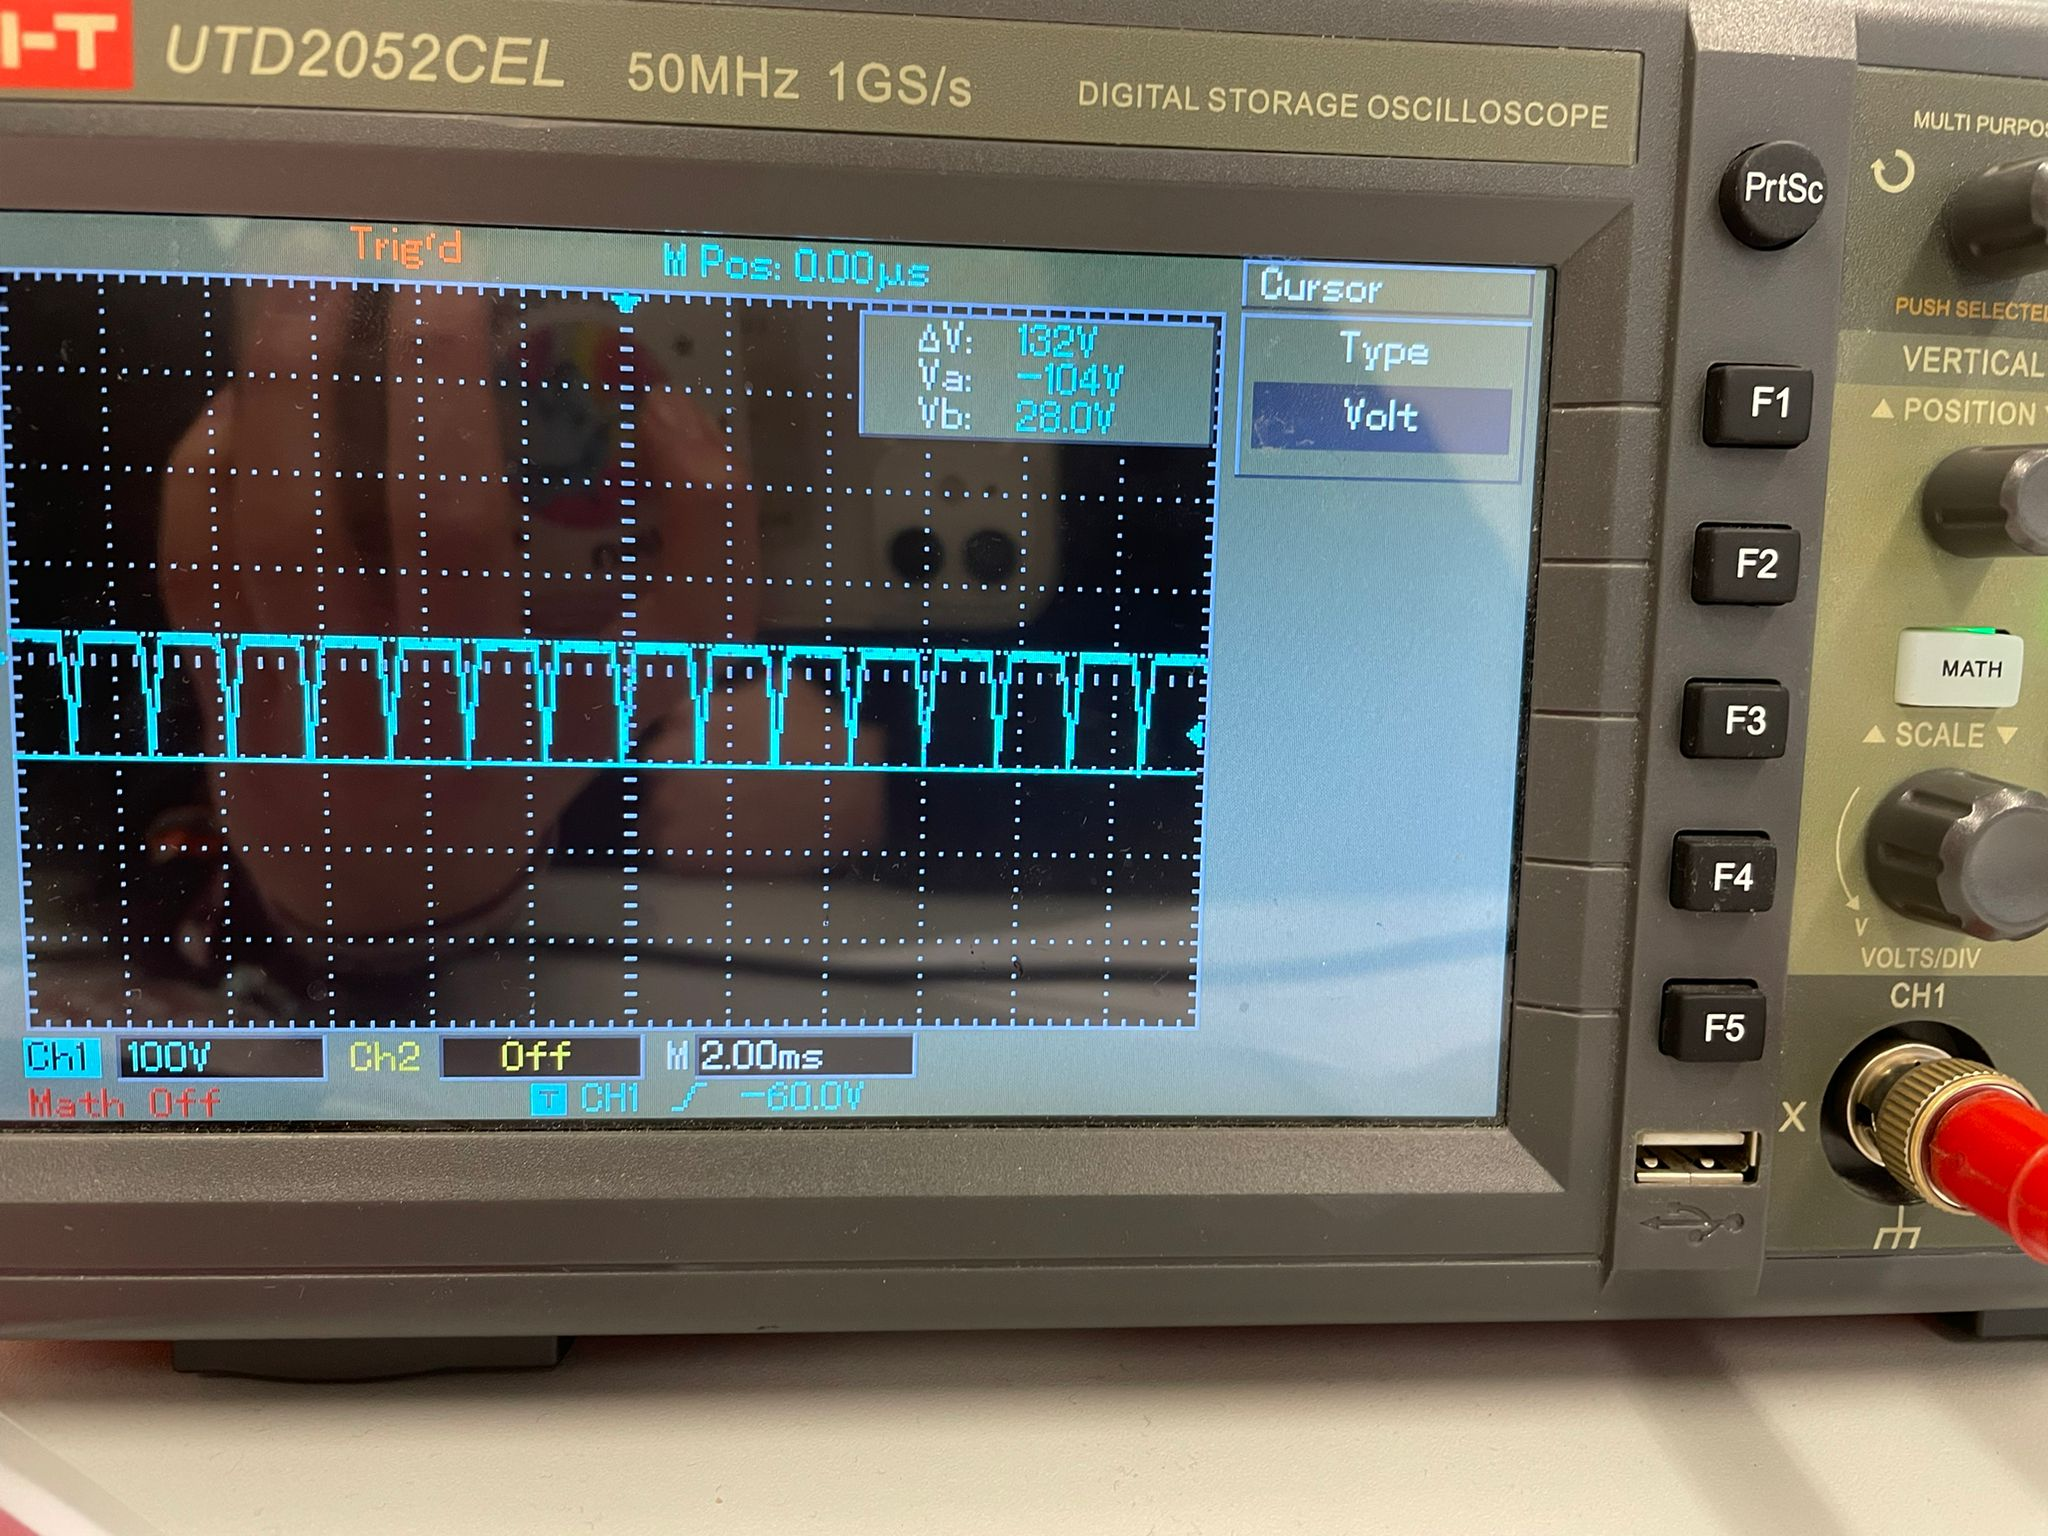
\includegraphics[scale=0.1]{content/norausch0.jpg}
    \caption{0° nicht verrauscht}
    \label{subfig:norausch0}
  \end{subfigure}
  \hfill
  \begin{subfigure}{0.48\textwidth}
    \centering
    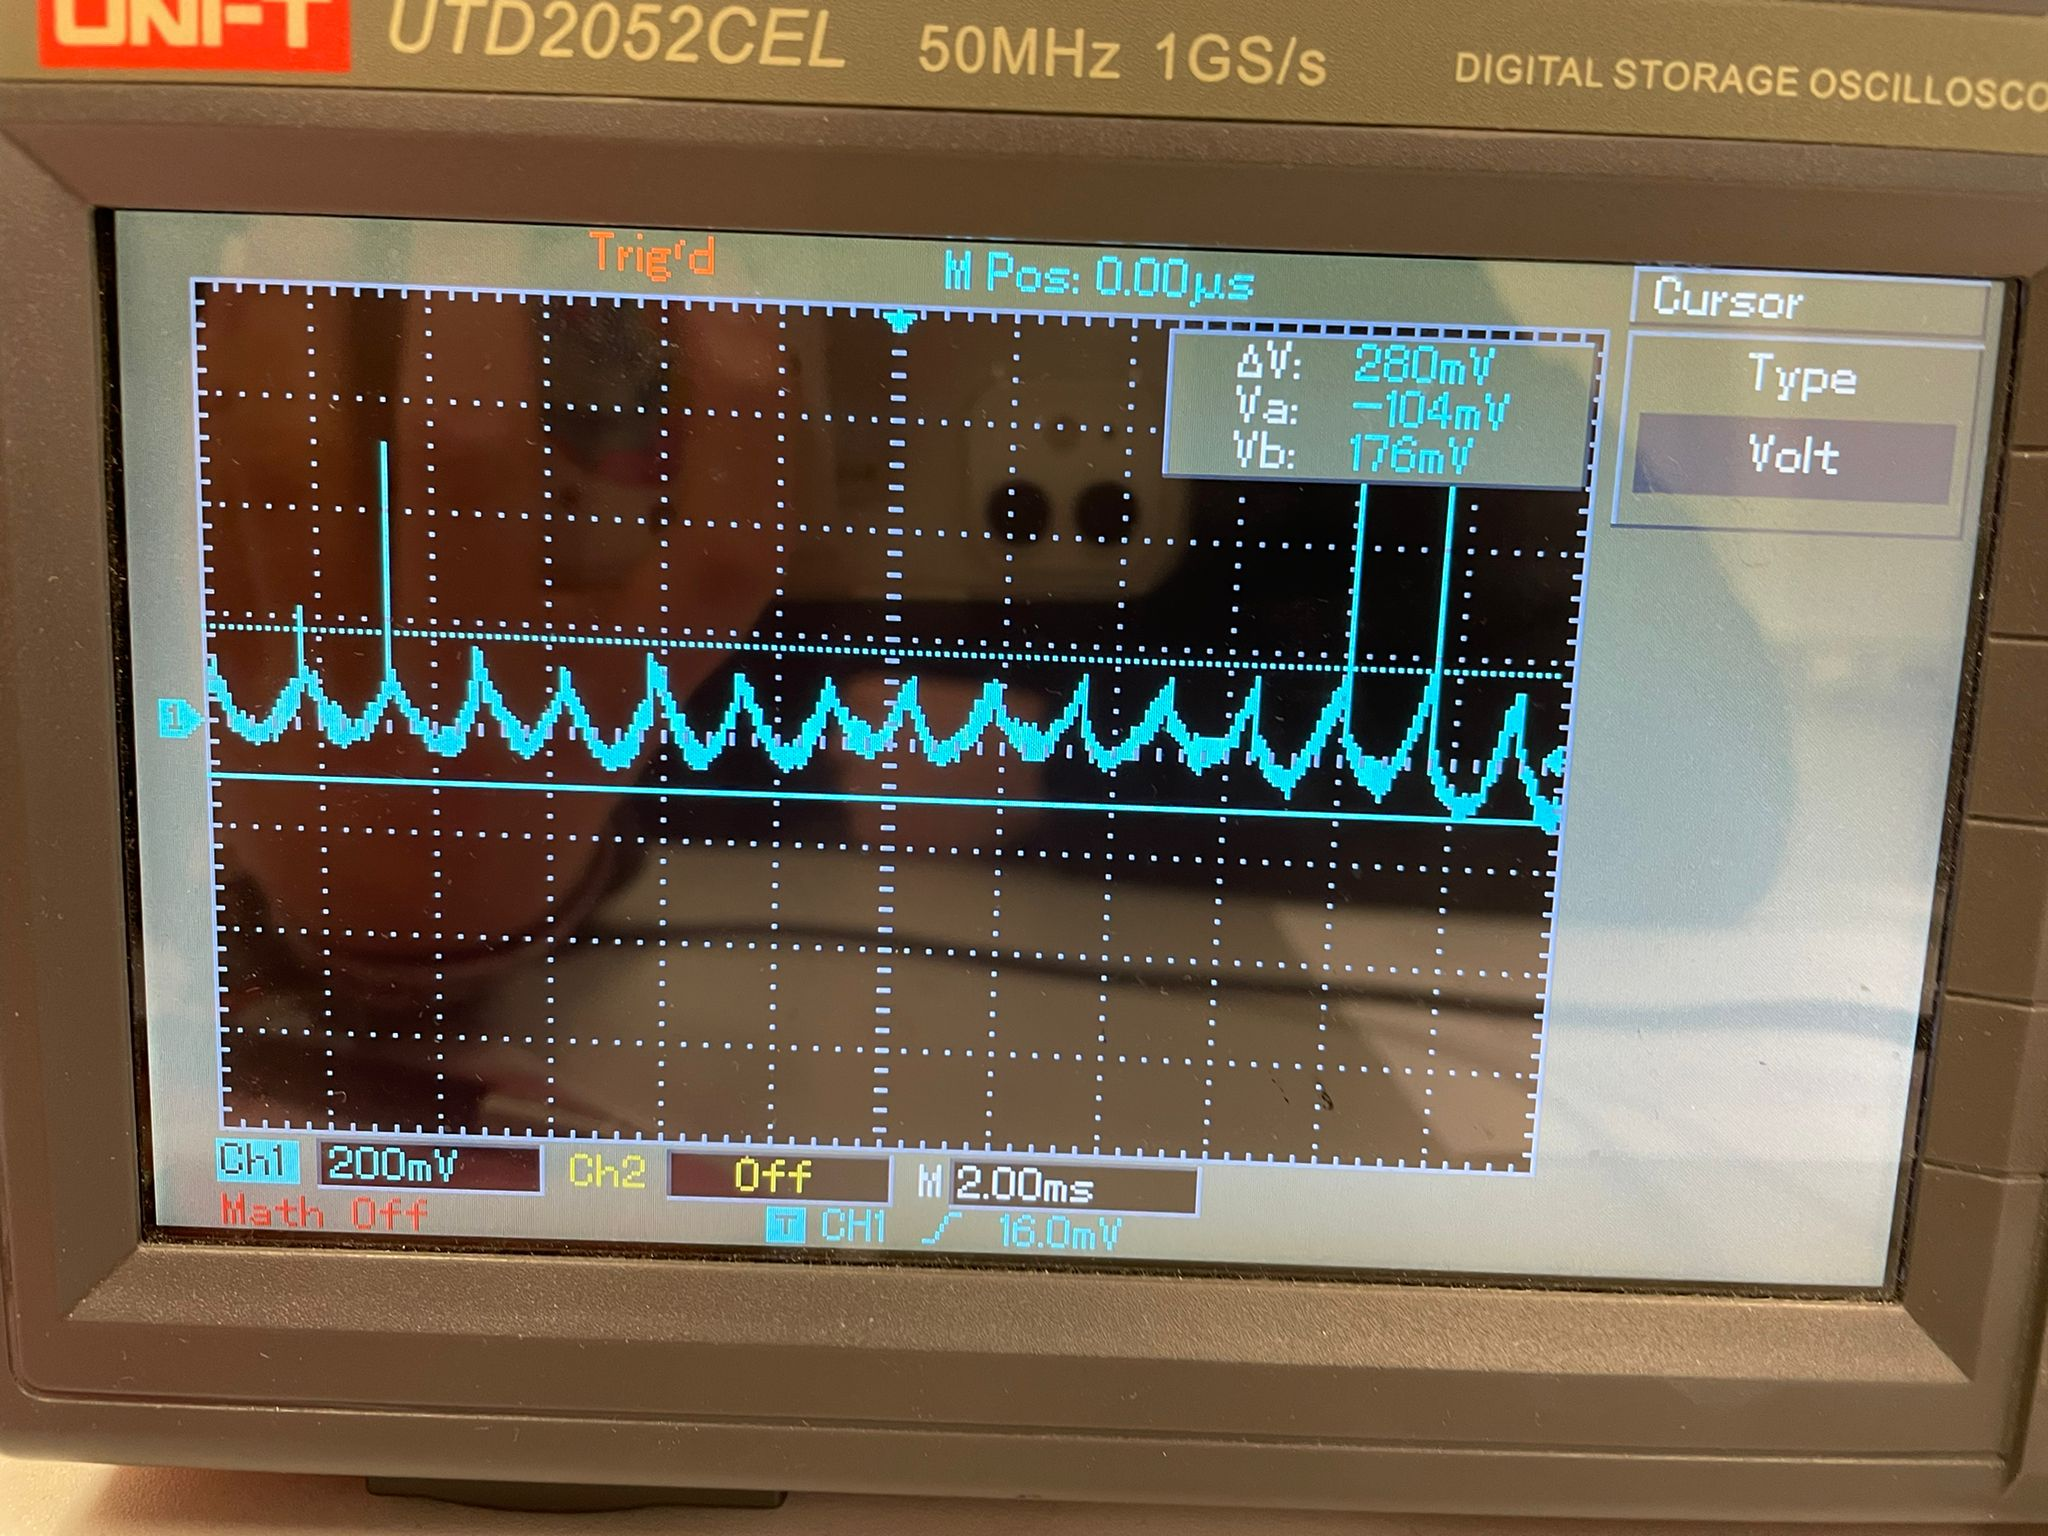
\includegraphics[scale=0.1]{content/rausch0.jpg}
    \caption{0° verrauscht}
    \label{subfig:rausch0}
  \end{subfigure}
\end{figure}
\begin{figure}[H]  
  \centering
  \begin{subfigure}{0.48\textwidth}
    \centering
    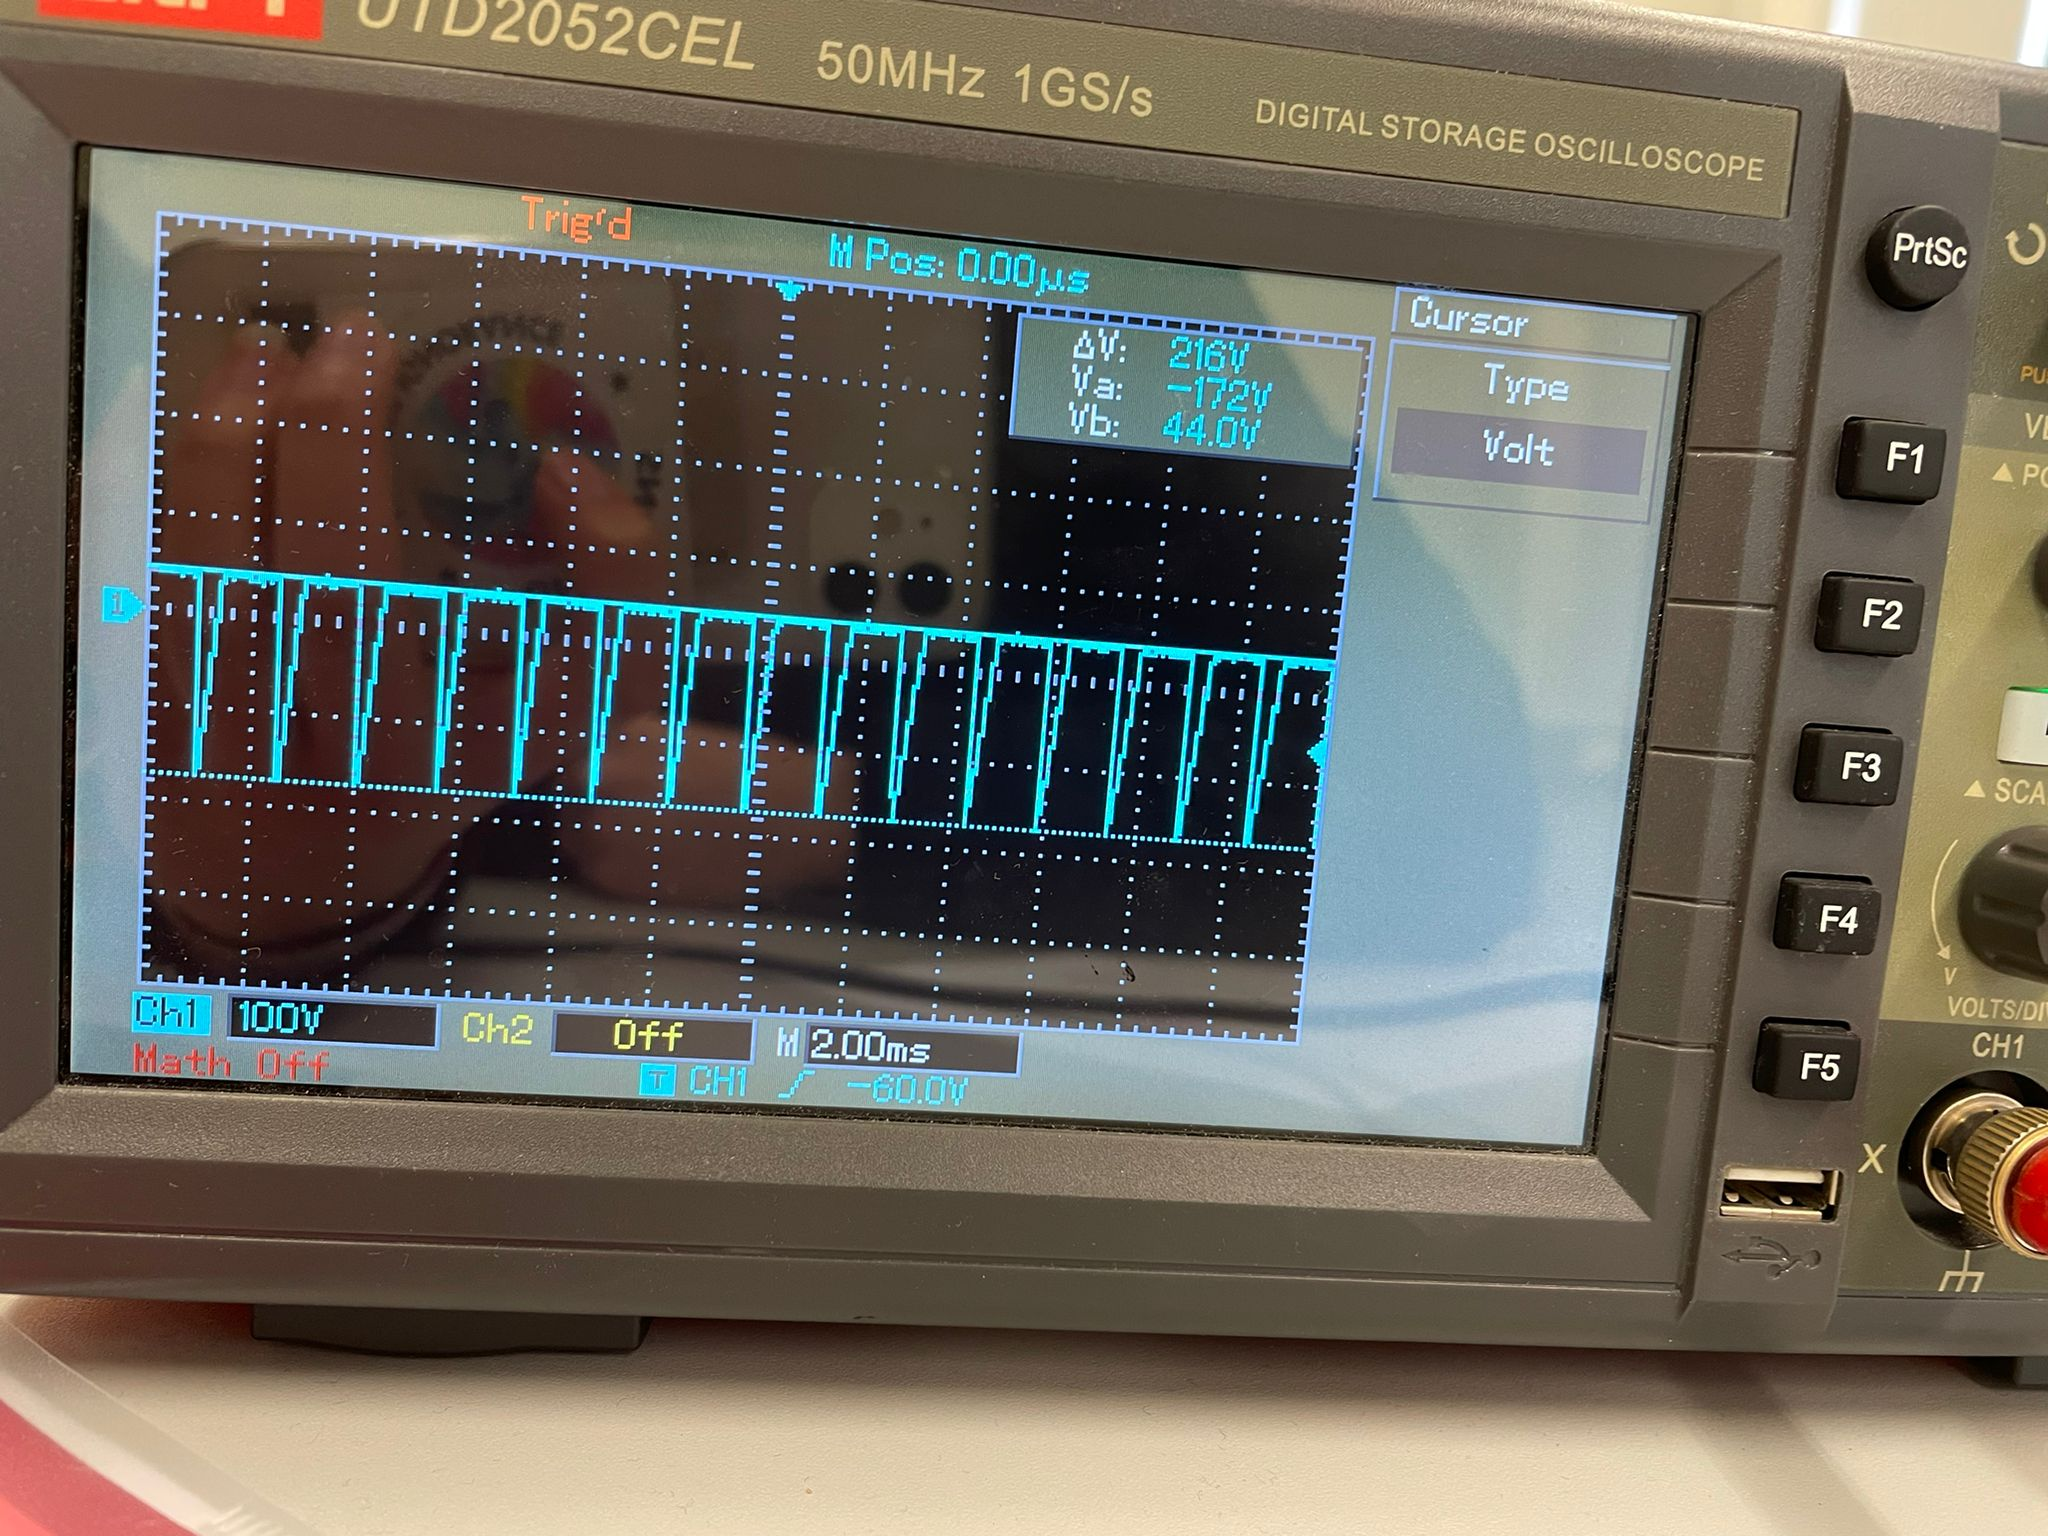
\includegraphics[scale=0.1]{content/norausch30.jpg}
    \caption{30° nicht verrauscht}
    \label{subfig:norausch30}
  \end{subfigure}
  \hfill
  \begin{subfigure}{0.48\textwidth}
    \centering
    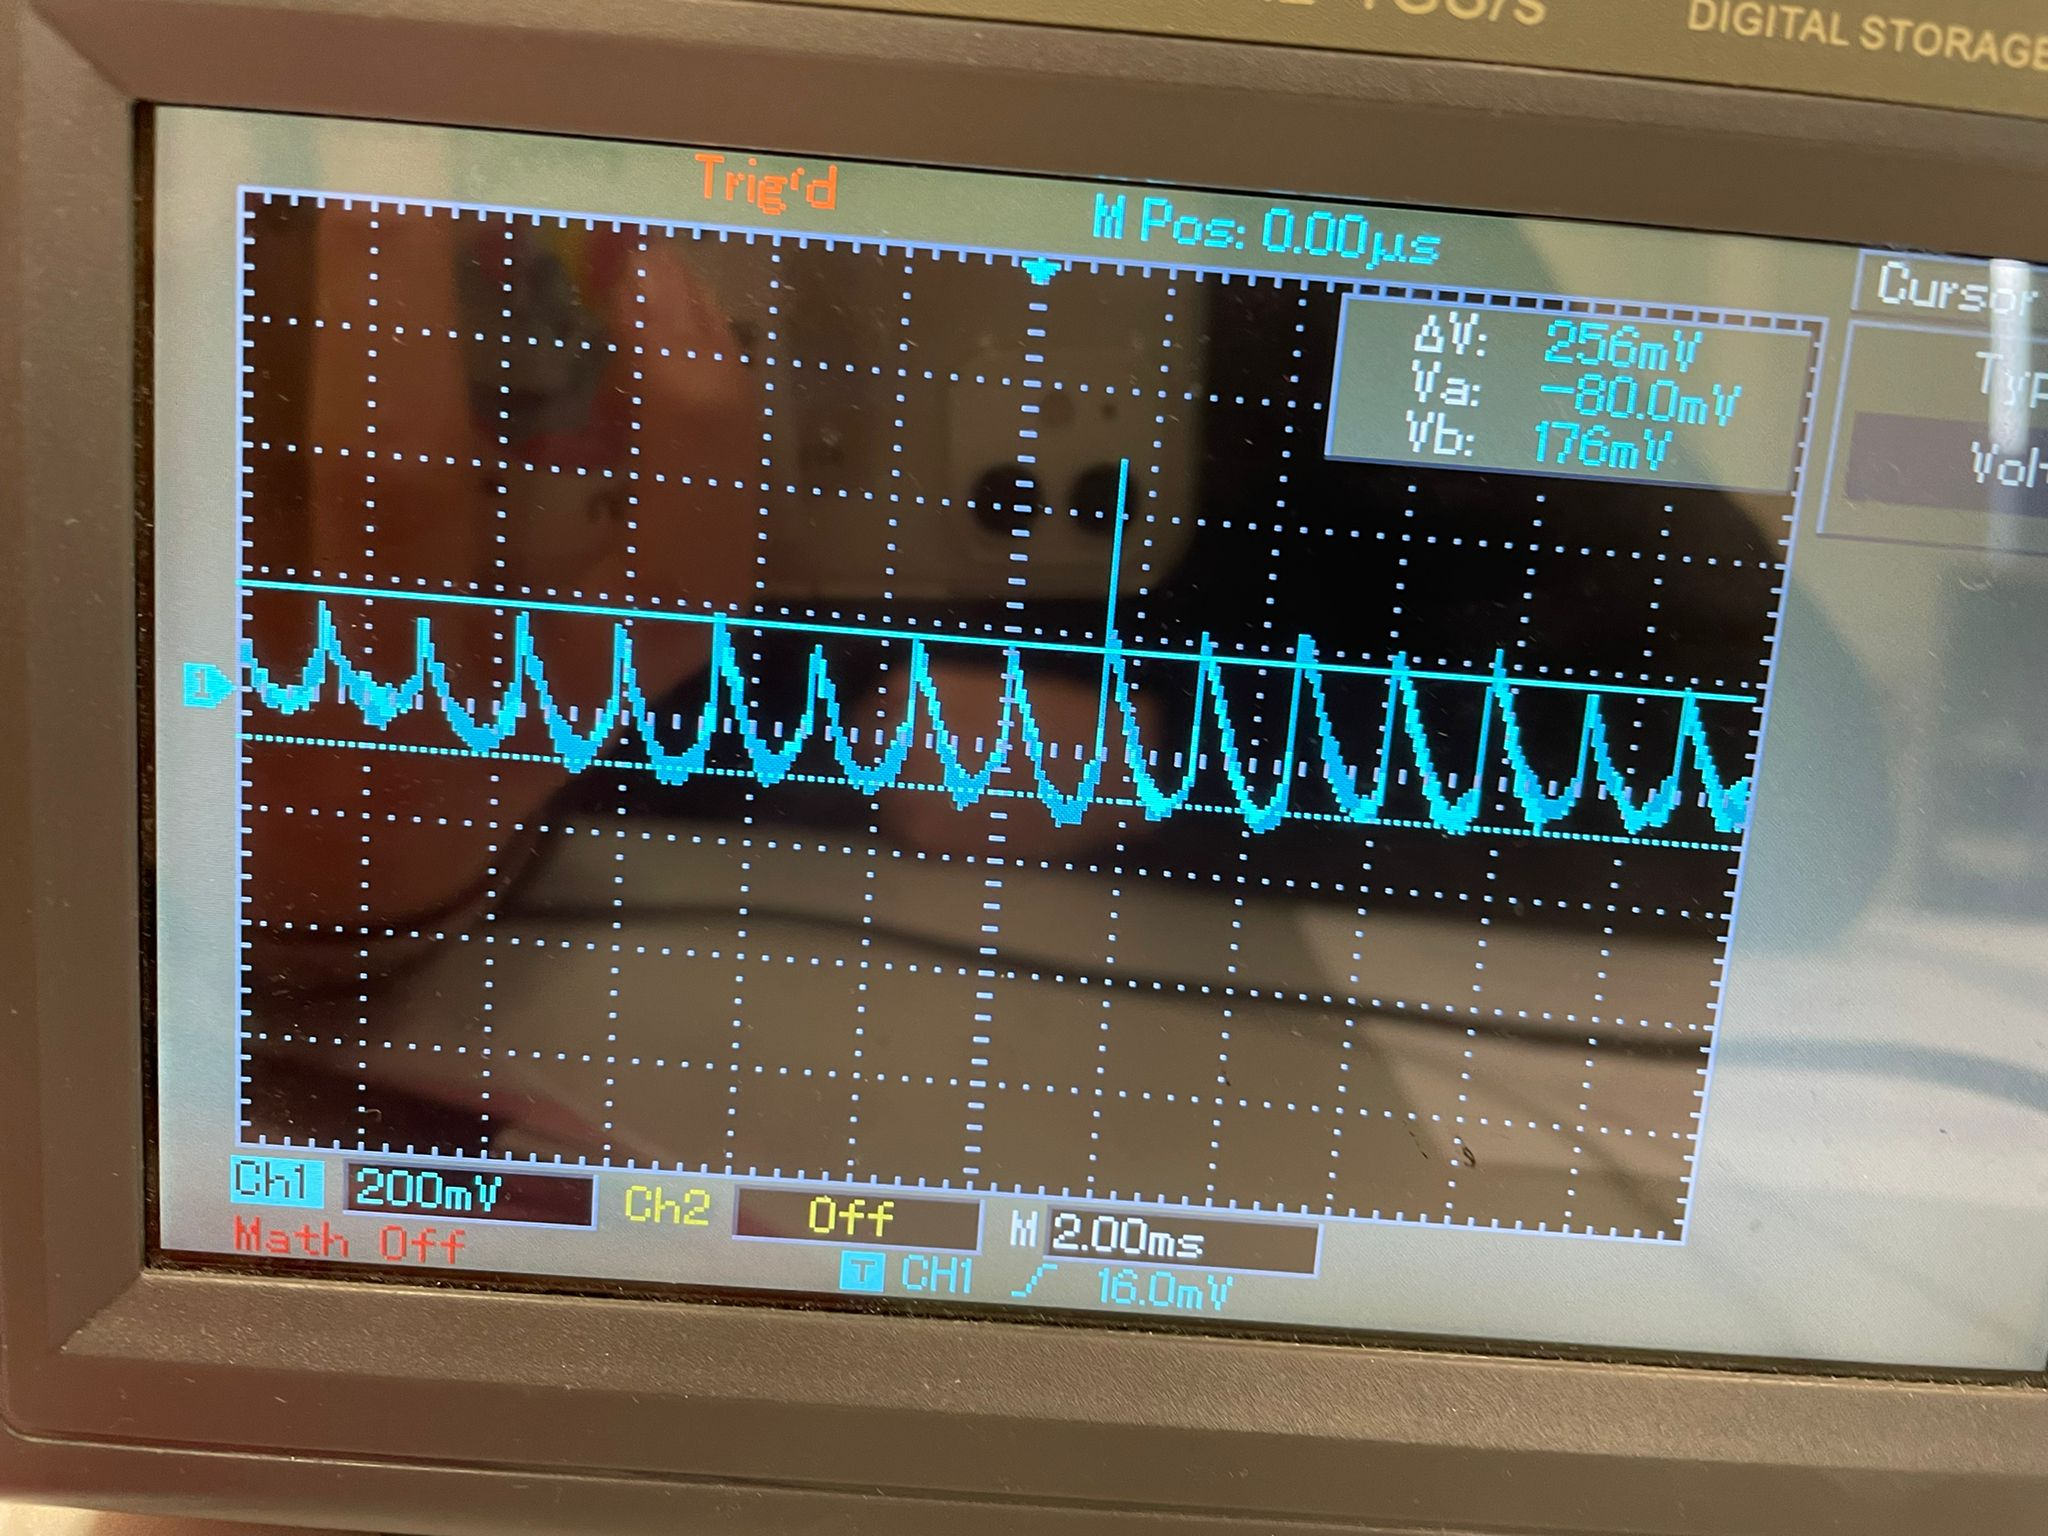
\includegraphics[scale=0.1]{content/rausch30.jpg}
    \caption{30° verrauscht}
    \label{subfig:rausch30}
  \end{subfigure}
\end{figure}
\begin{figure}[H]  
  \centering
  \begin{subfigure}{0.48\textwidth}
    \centering
    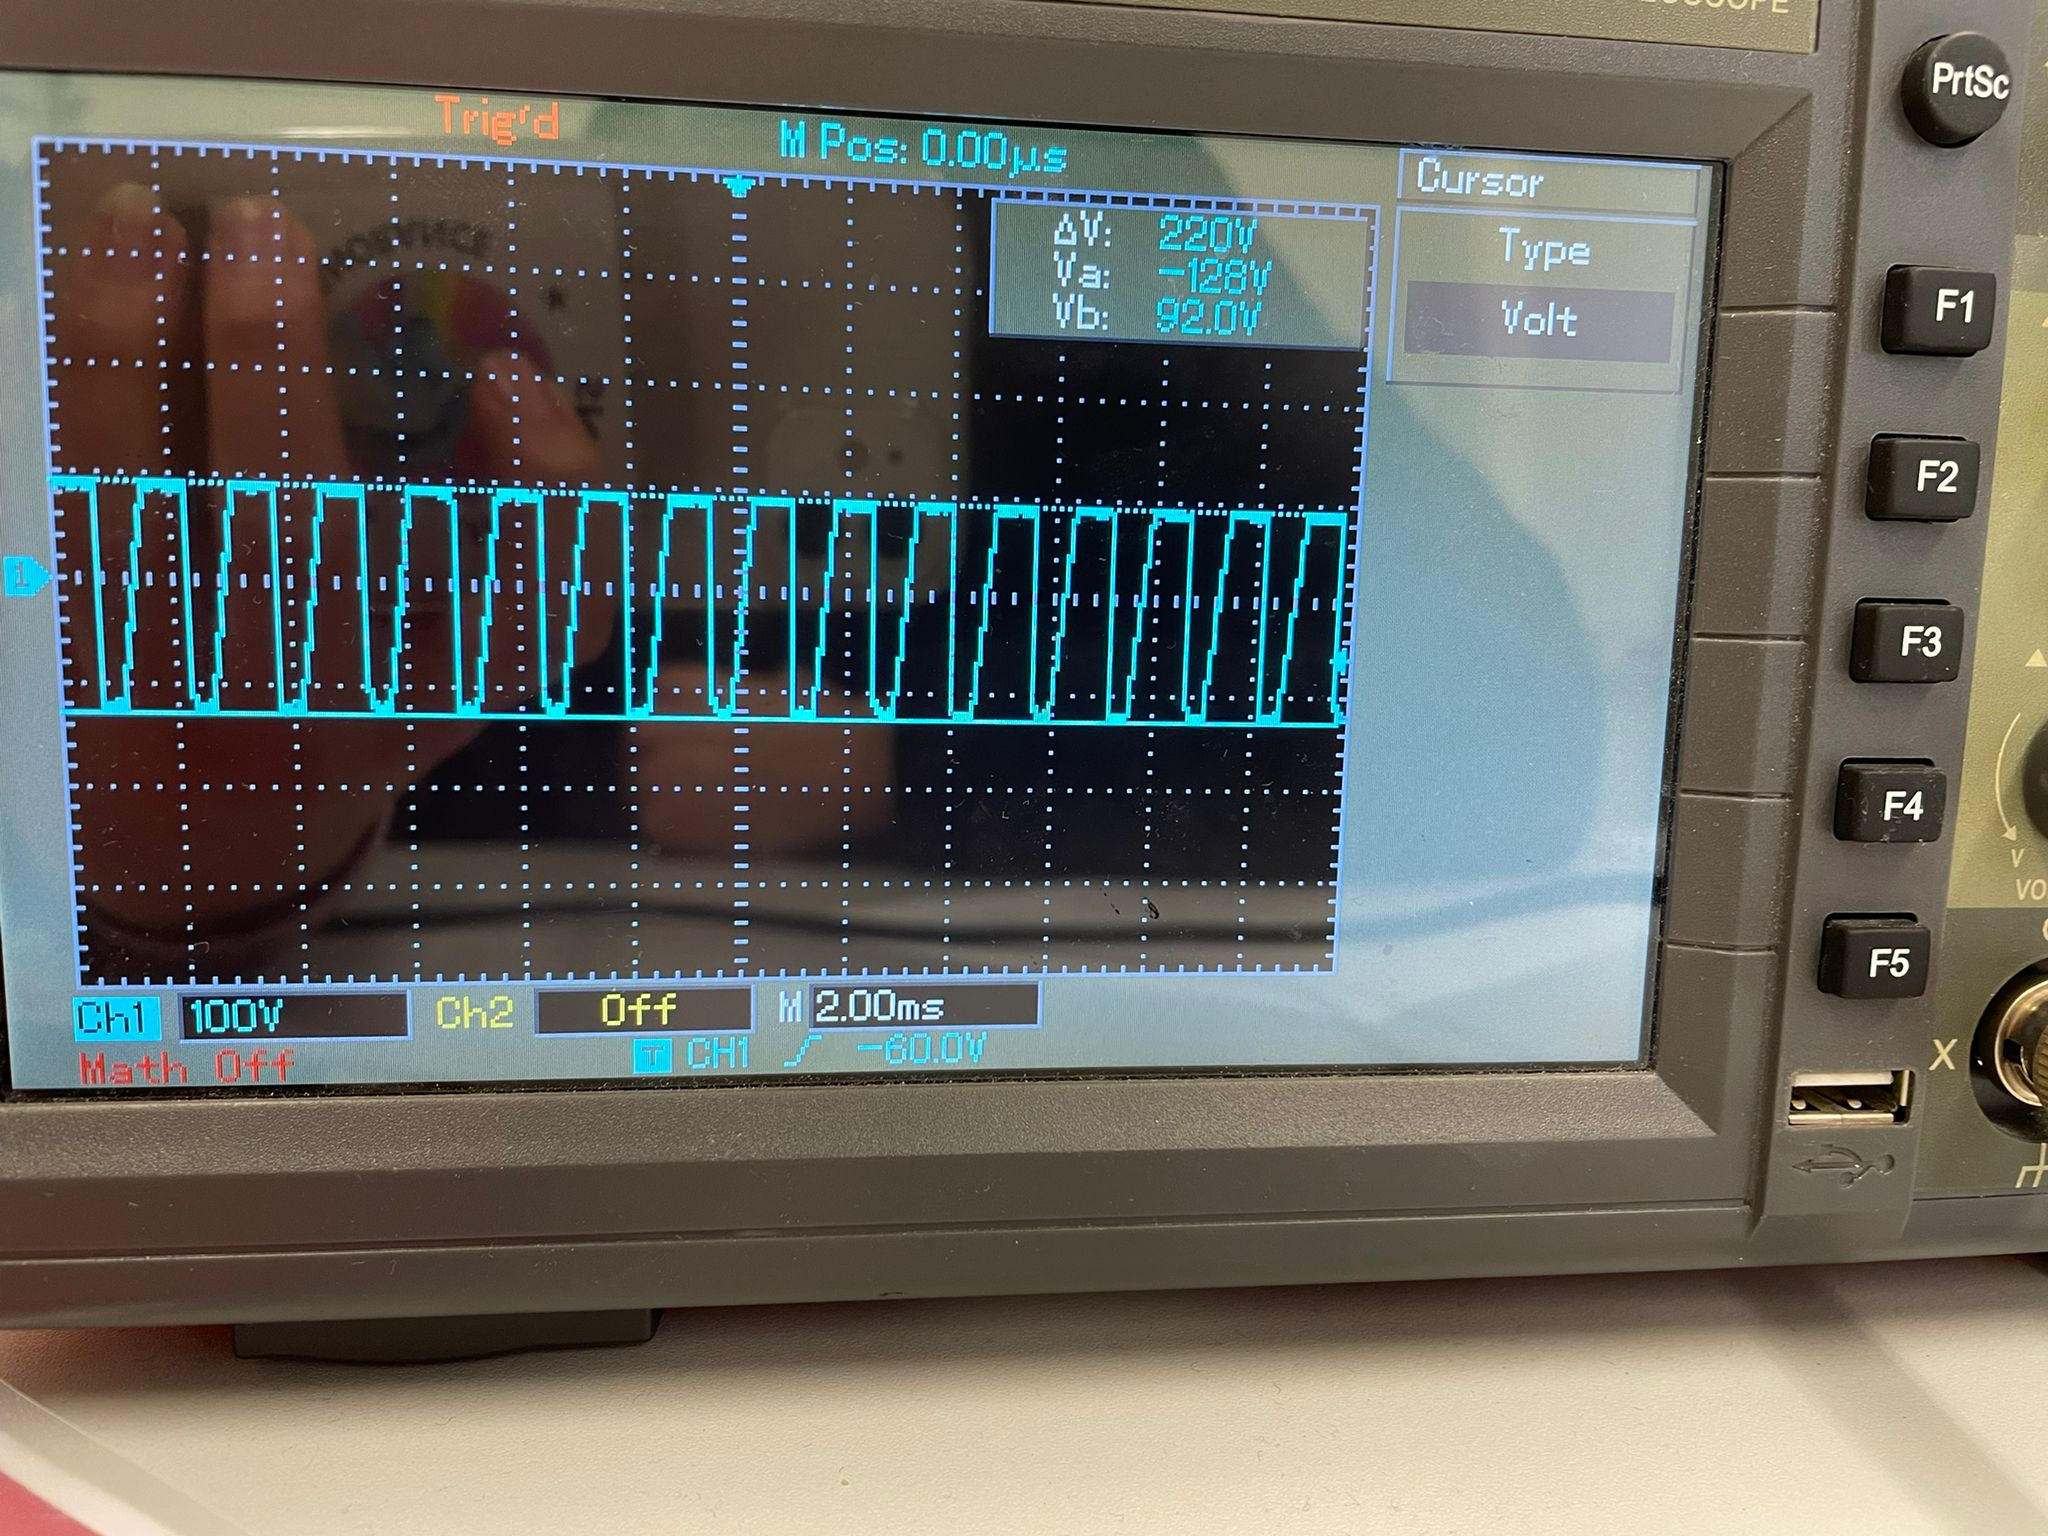
\includegraphics[scale=0.1]{content/norausch60.jpg}
    \caption{60° nicht verrauscht}
    \label{subfig:norausch60}
  \end{subfigure}
  \hfill
  \begin{subfigure}{0.48\textwidth}
    \centering
    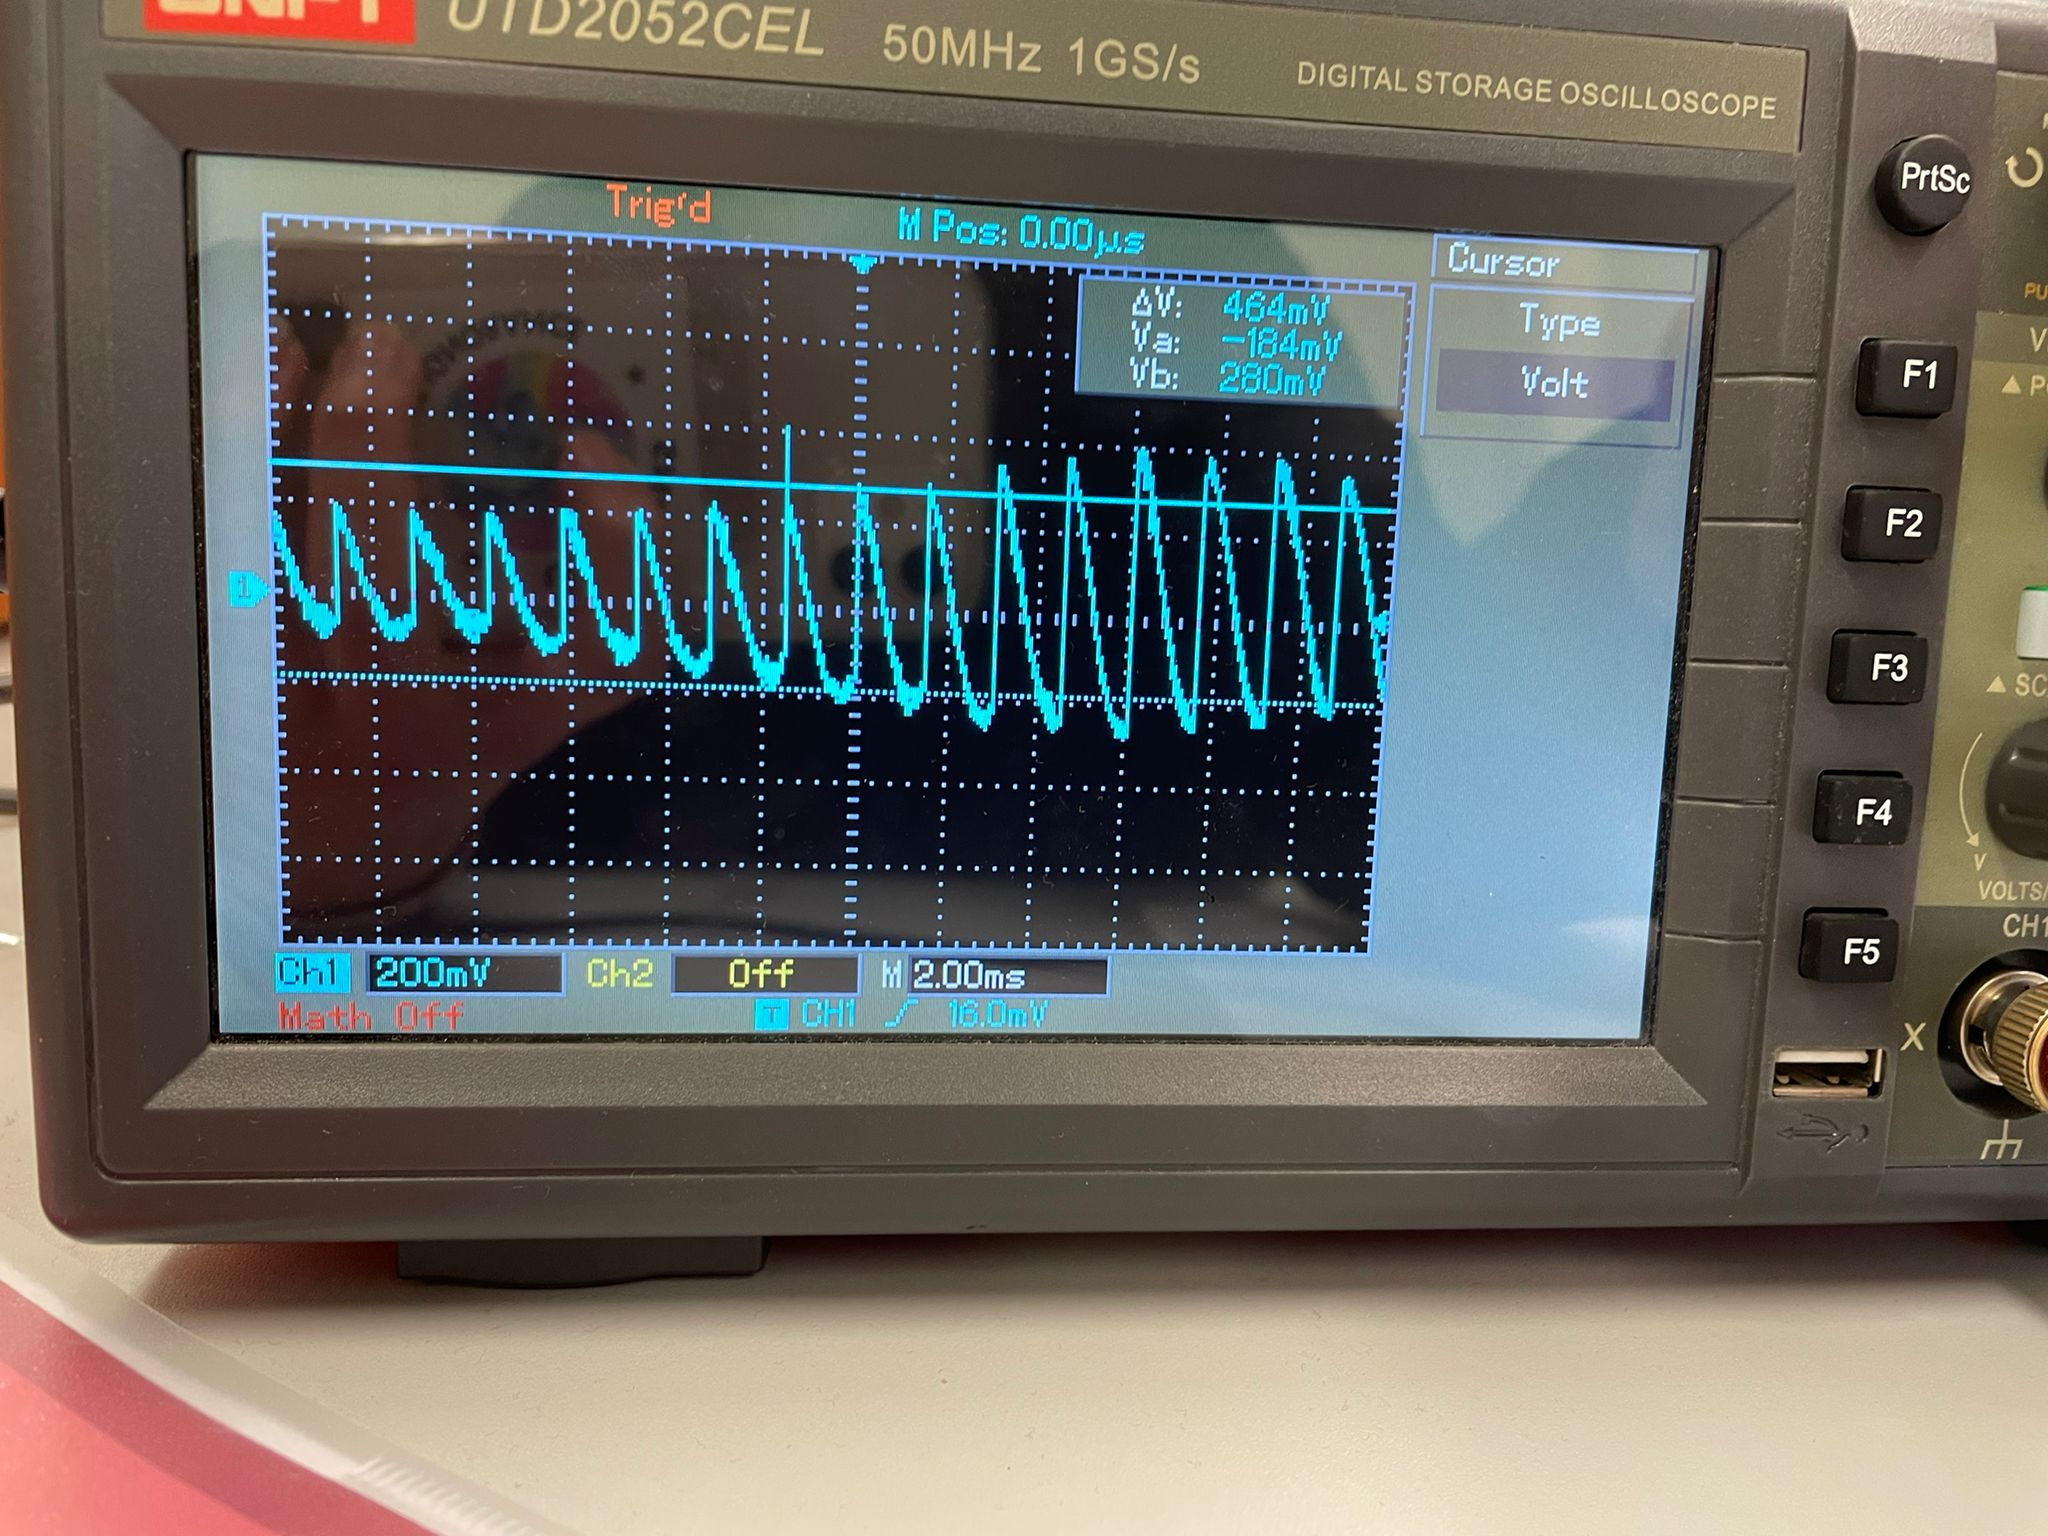
\includegraphics[scale=0.1]{content/rausch60.jpg}
    \caption{60° verrauscht}
    \label{subfig:rausch60}
  \end{subfigure}
\end{figure}
\begin{figure}[H]  
  \centering
  \begin{subfigure}{0.48\textwidth}
    \centering
    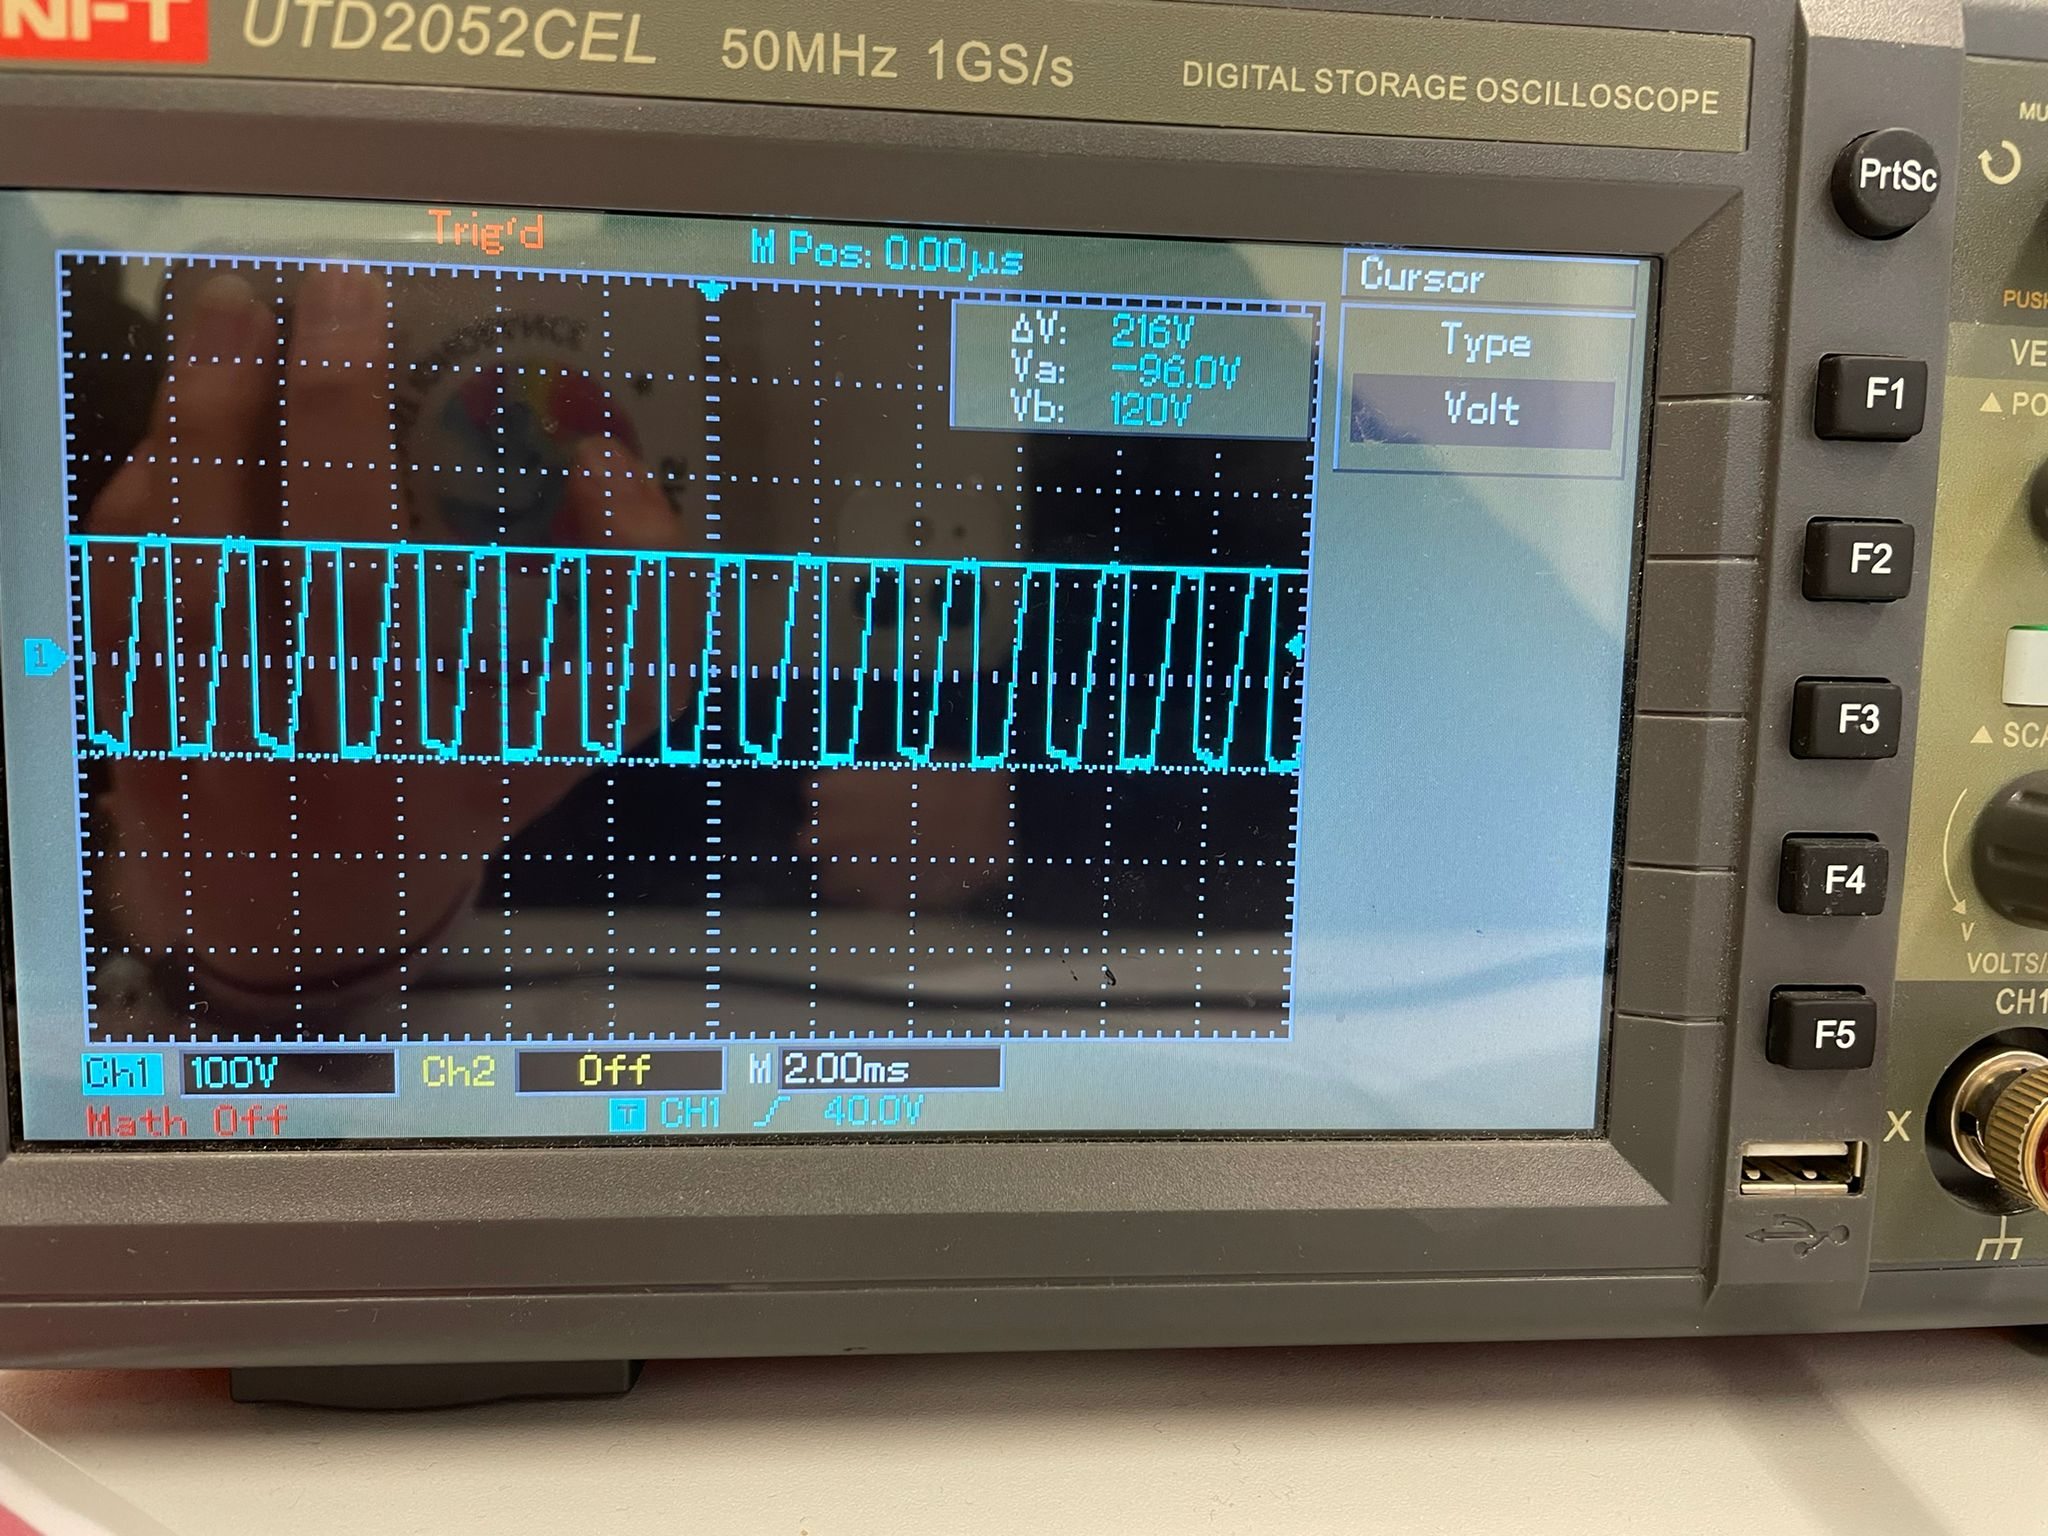
\includegraphics[scale=0.1]{content/norausch90.jpg}
    \caption{90° nicht verrauscht}
    \label{subfig:norausch90}
  \end{subfigure}
  \hfill
  \begin{subfigure}{0.48\textwidth}
    \centering
    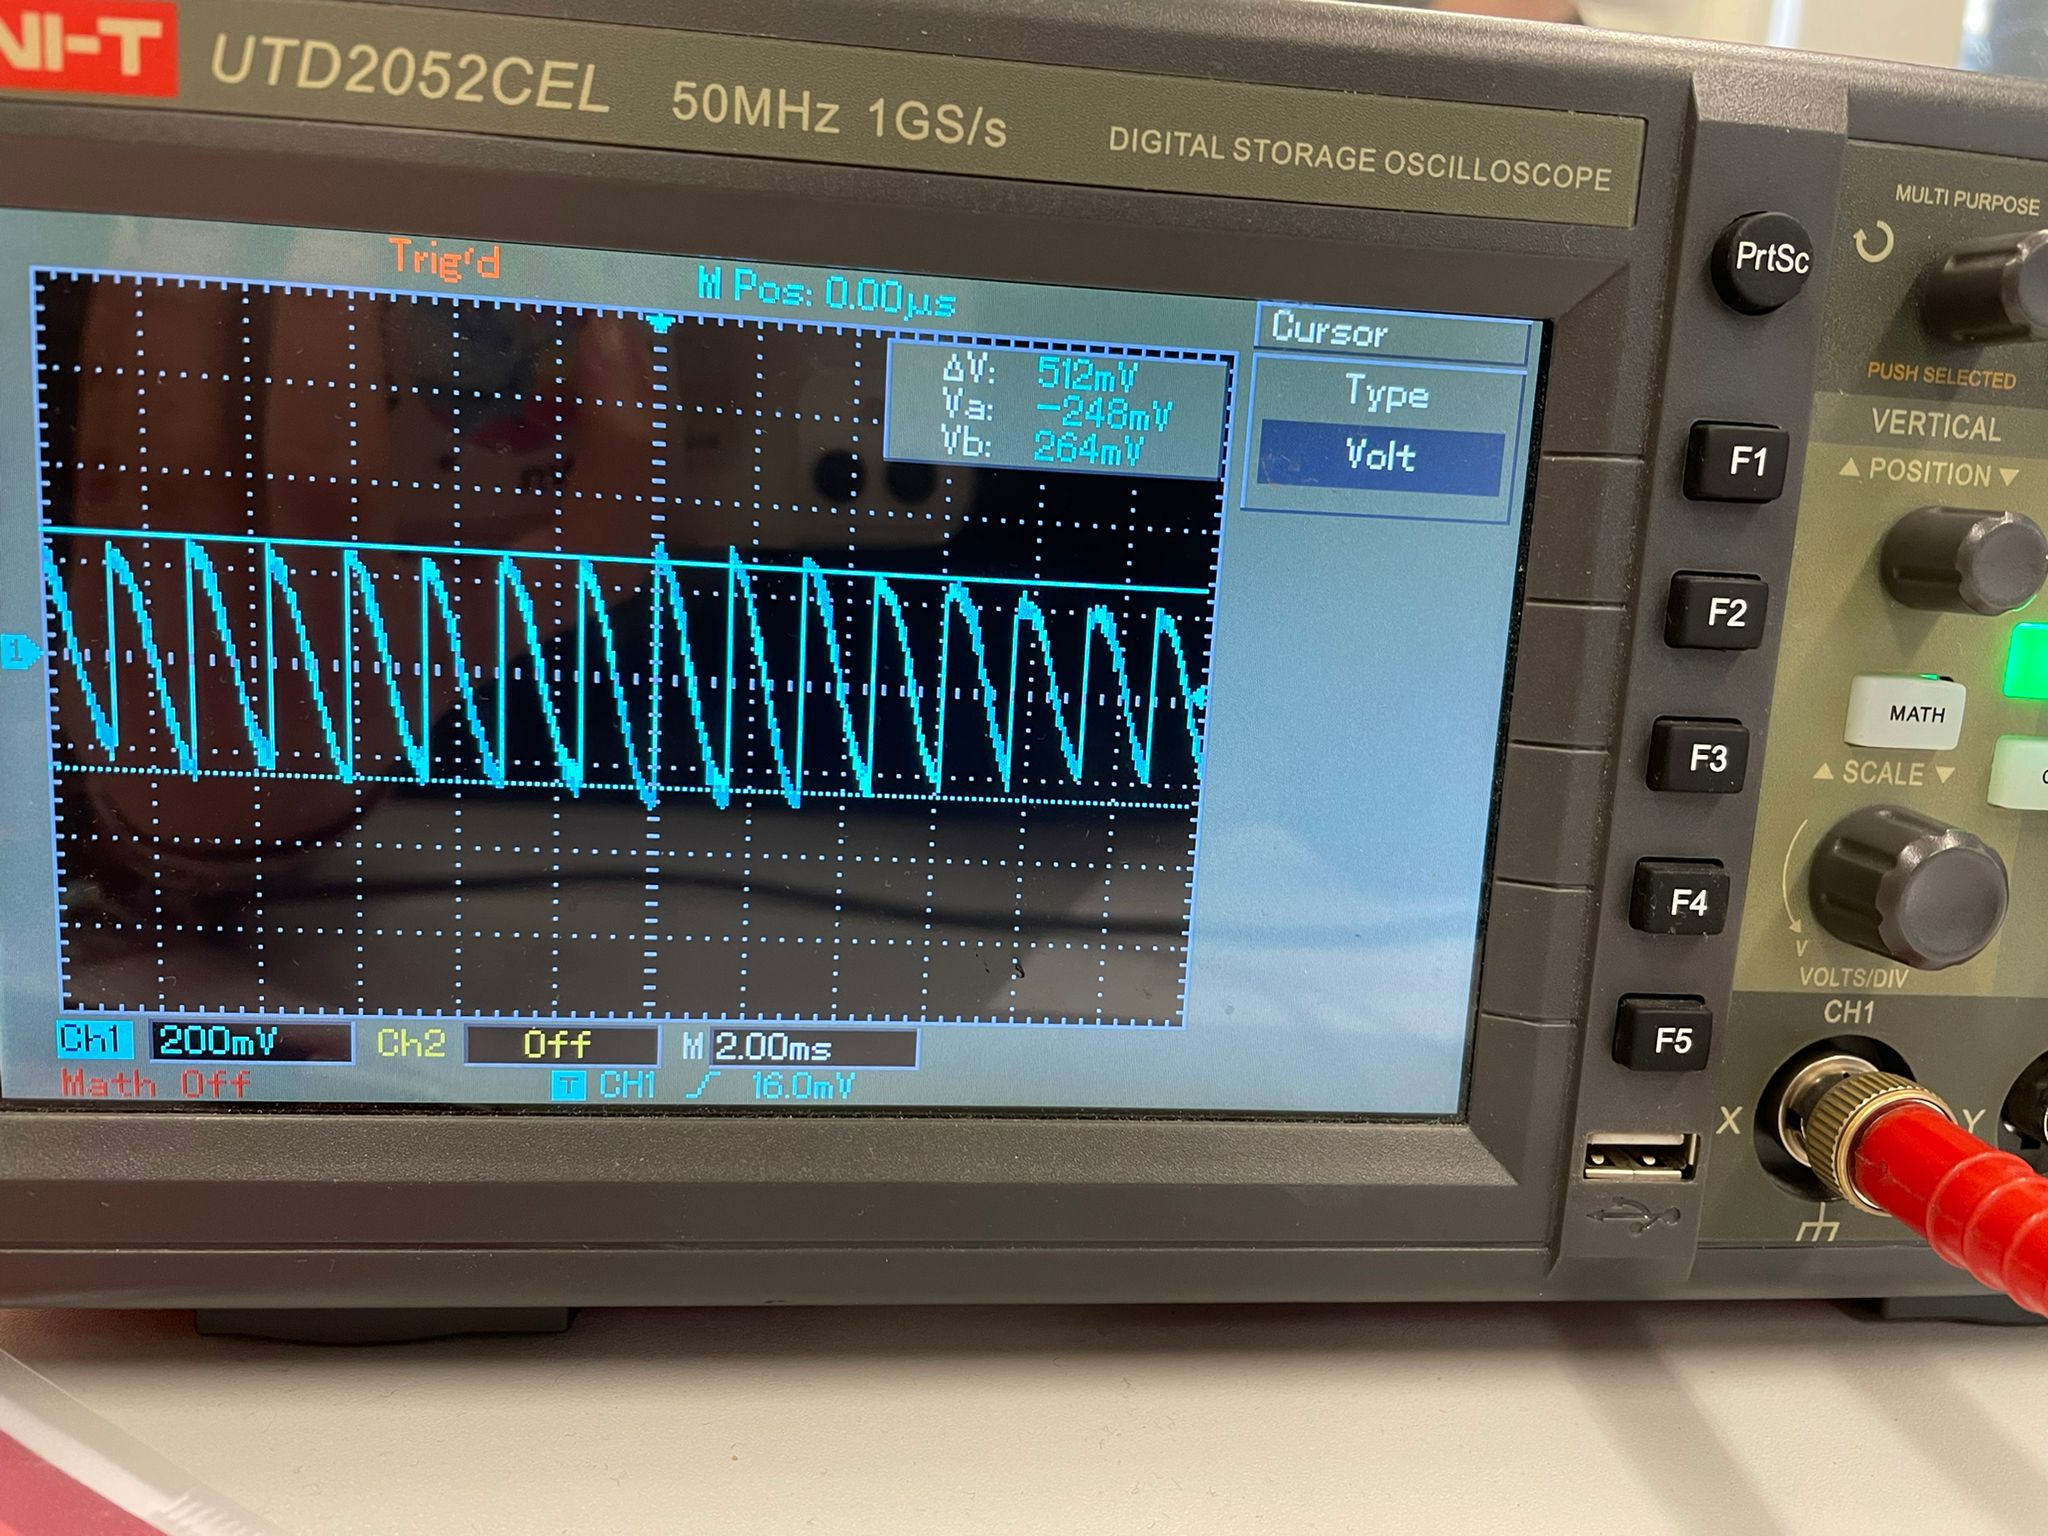
\includegraphics[scale=0.1]{content/rausch90.jpg}
    \caption{90° verrauscht}
    \label{subfig:rausch90}
  \end{subfigure}
\end{figure}
\begin{figure}[H]  
  \centering
  \begin{subfigure}{0.48\textwidth}
    \centering
    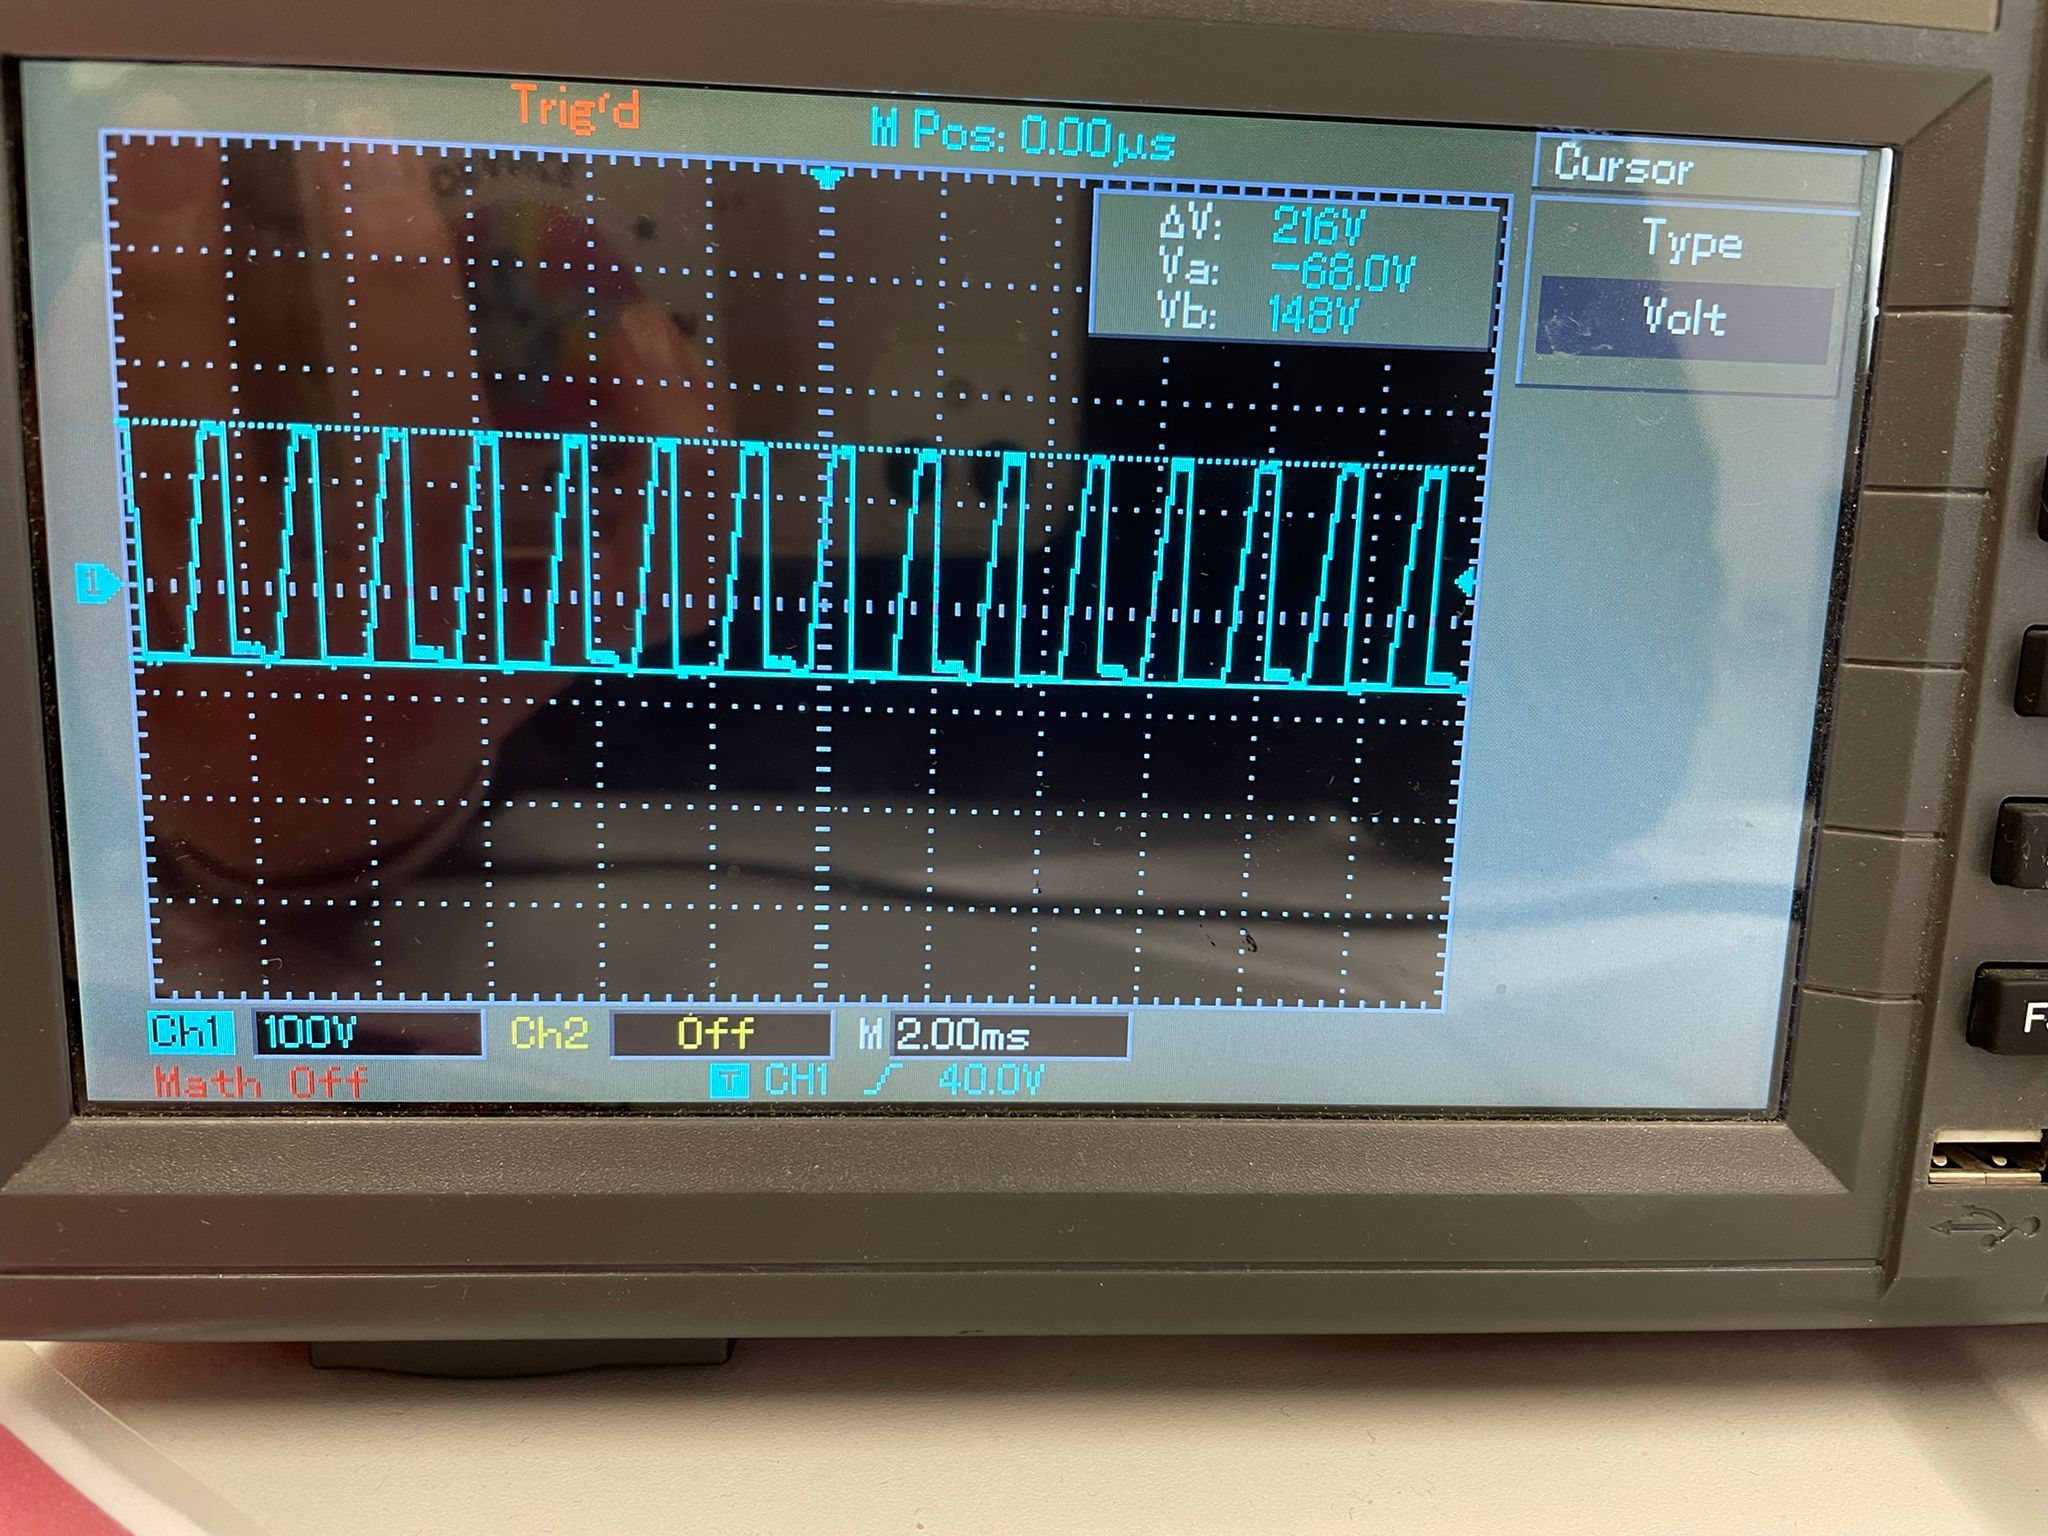
\includegraphics[scale=0.1]{content/norausch120.jpg}
    \caption{120° nicht verrauscht}
    \label{subfig:norausch120}
  \end{subfigure}
  \hfill
  \begin{subfigure}{0.48\textwidth}
    \centering
    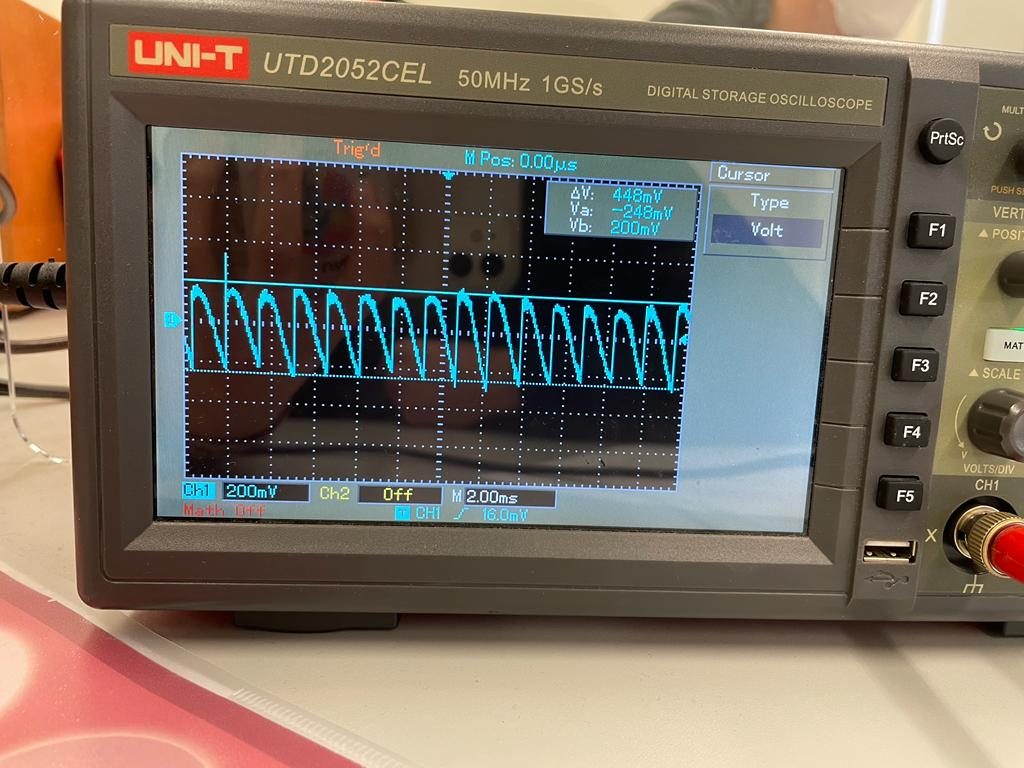
\includegraphics[scale=0.2]{content/rausch120.jpg}
    \caption{120° verrauscht}
    \label{subfig:rausch120}
  \end{subfigure}
\end{figure}
\begin{figure}[H]  
  \centering
  \begin{subfigure}{0.48\textwidth}
    \centering
    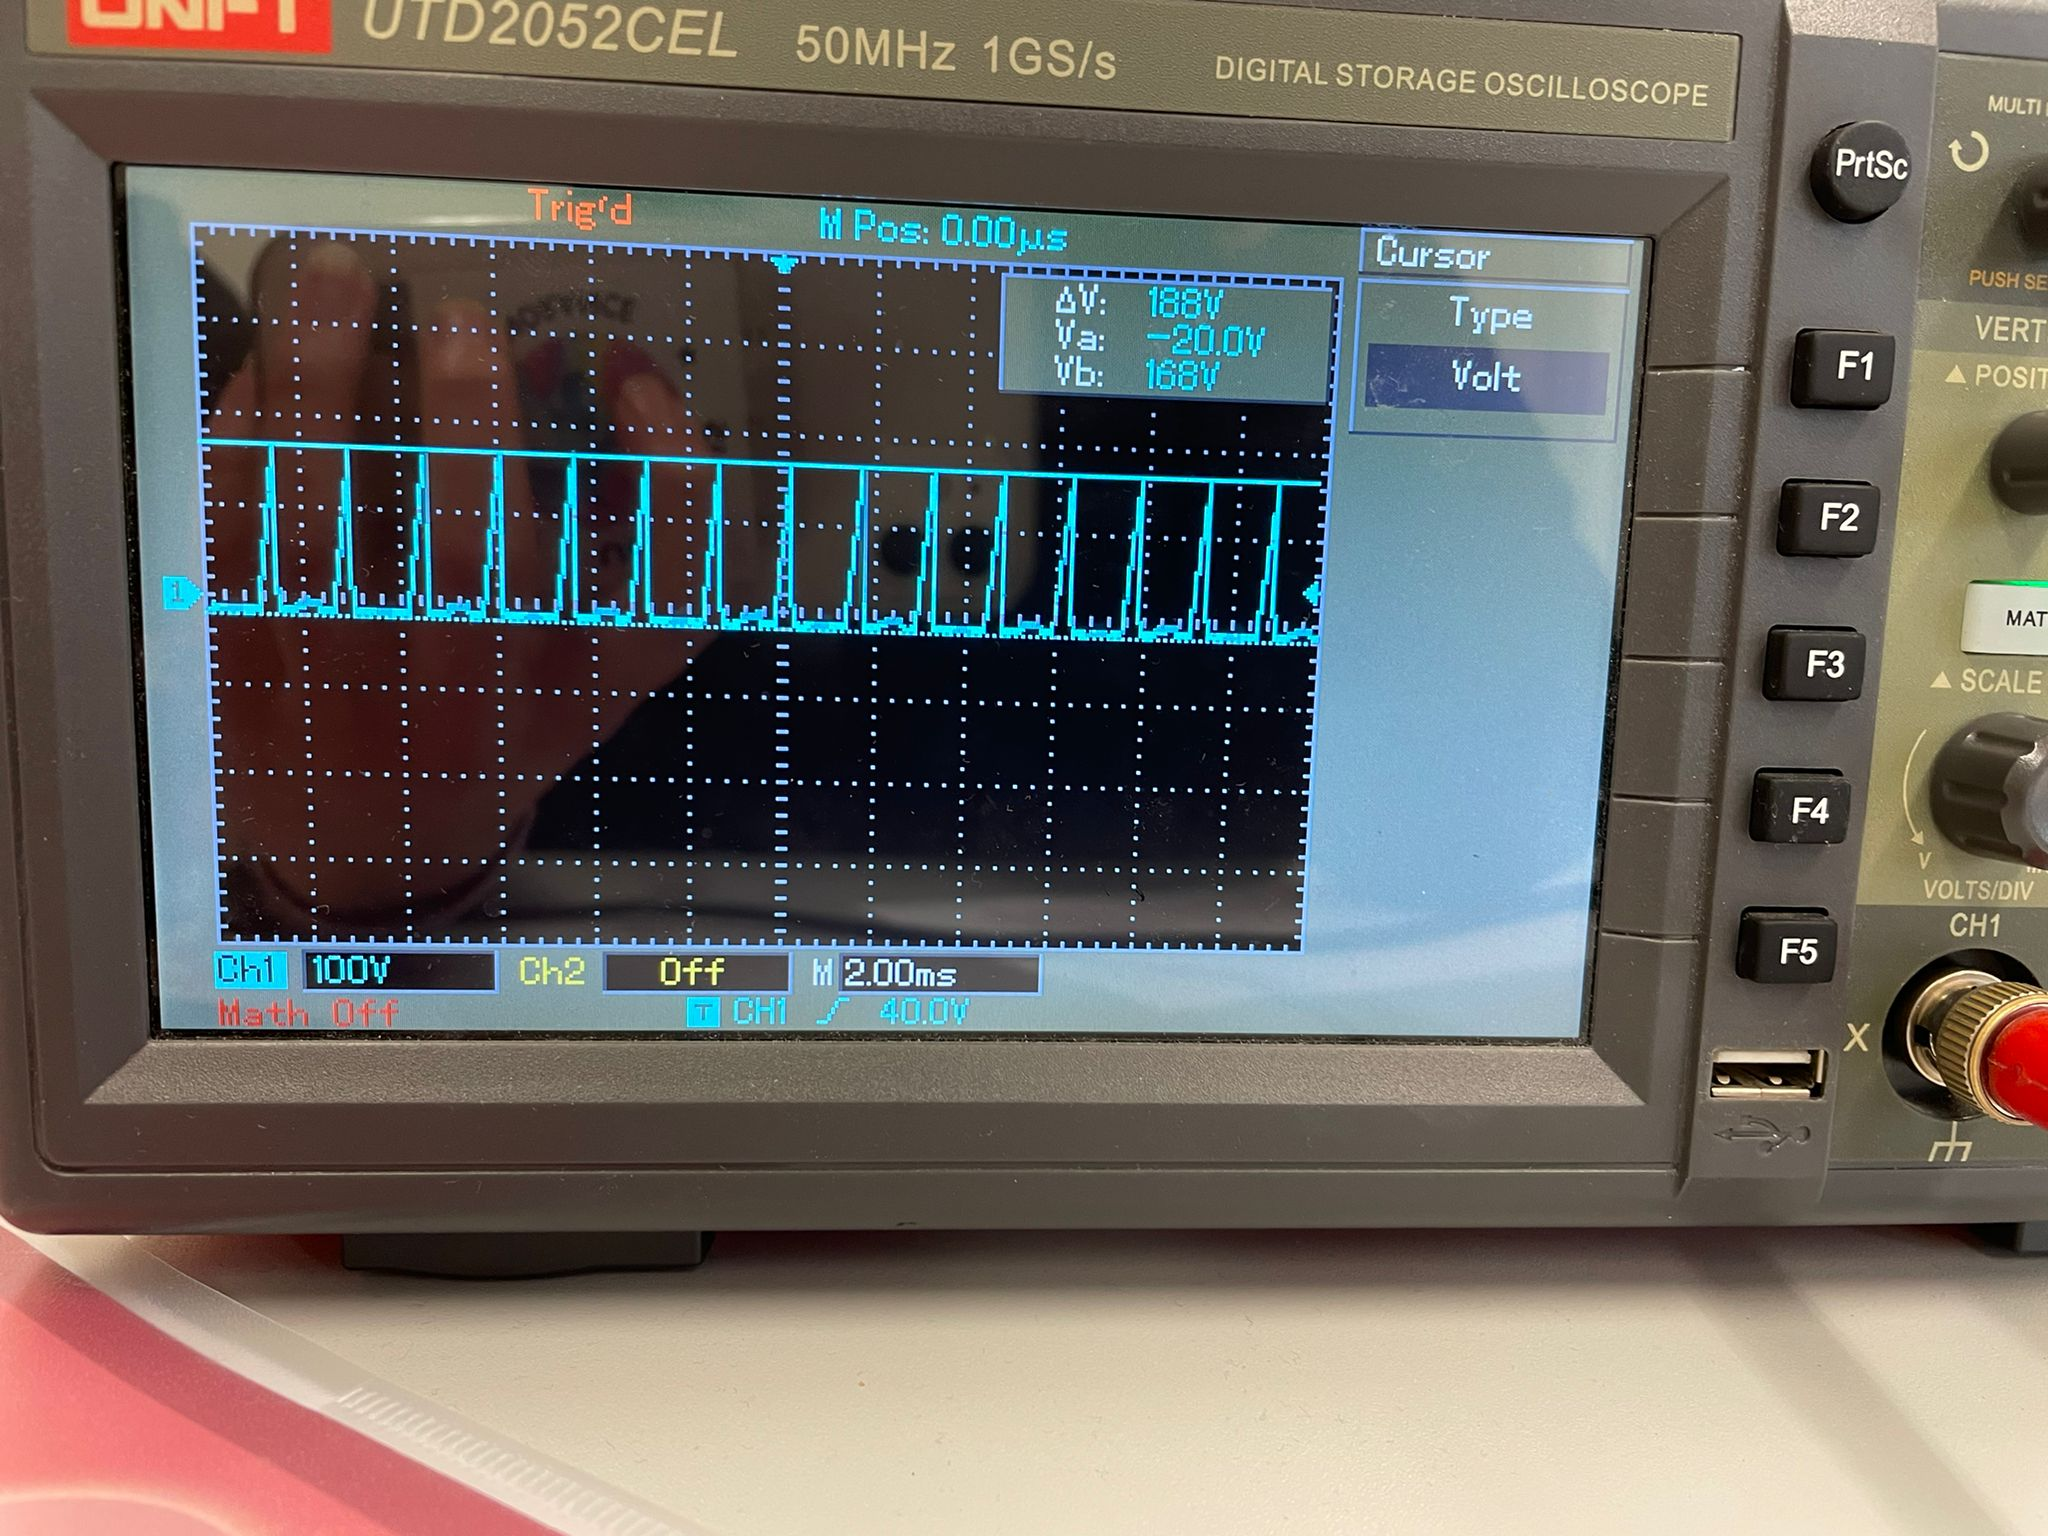
\includegraphics[scale=0.1]{content/norausch150.jpg}
    \caption{150° nicht verrauscht}
    \label{subfig:norausch150}
  \end{subfigure}
  \hfill
  \begin{subfigure}{0.48\textwidth}
    \centering
    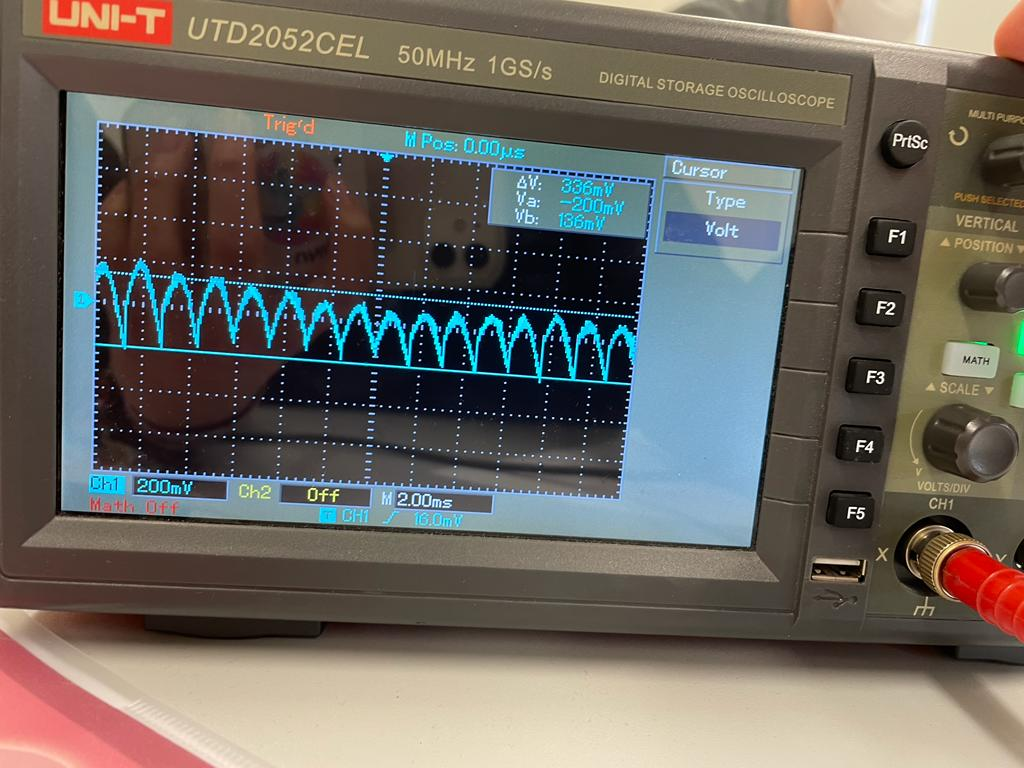
\includegraphics[scale=0.2]{content/rausch150.jpg}
    \caption{150° verrauscht}
    \label{subfig:rausch150}
  \end{subfigure}
\end{figure}
\begin{figure}[H]  
  \centering
  \begin{subfigure}{0.48\textwidth}
    \centering
    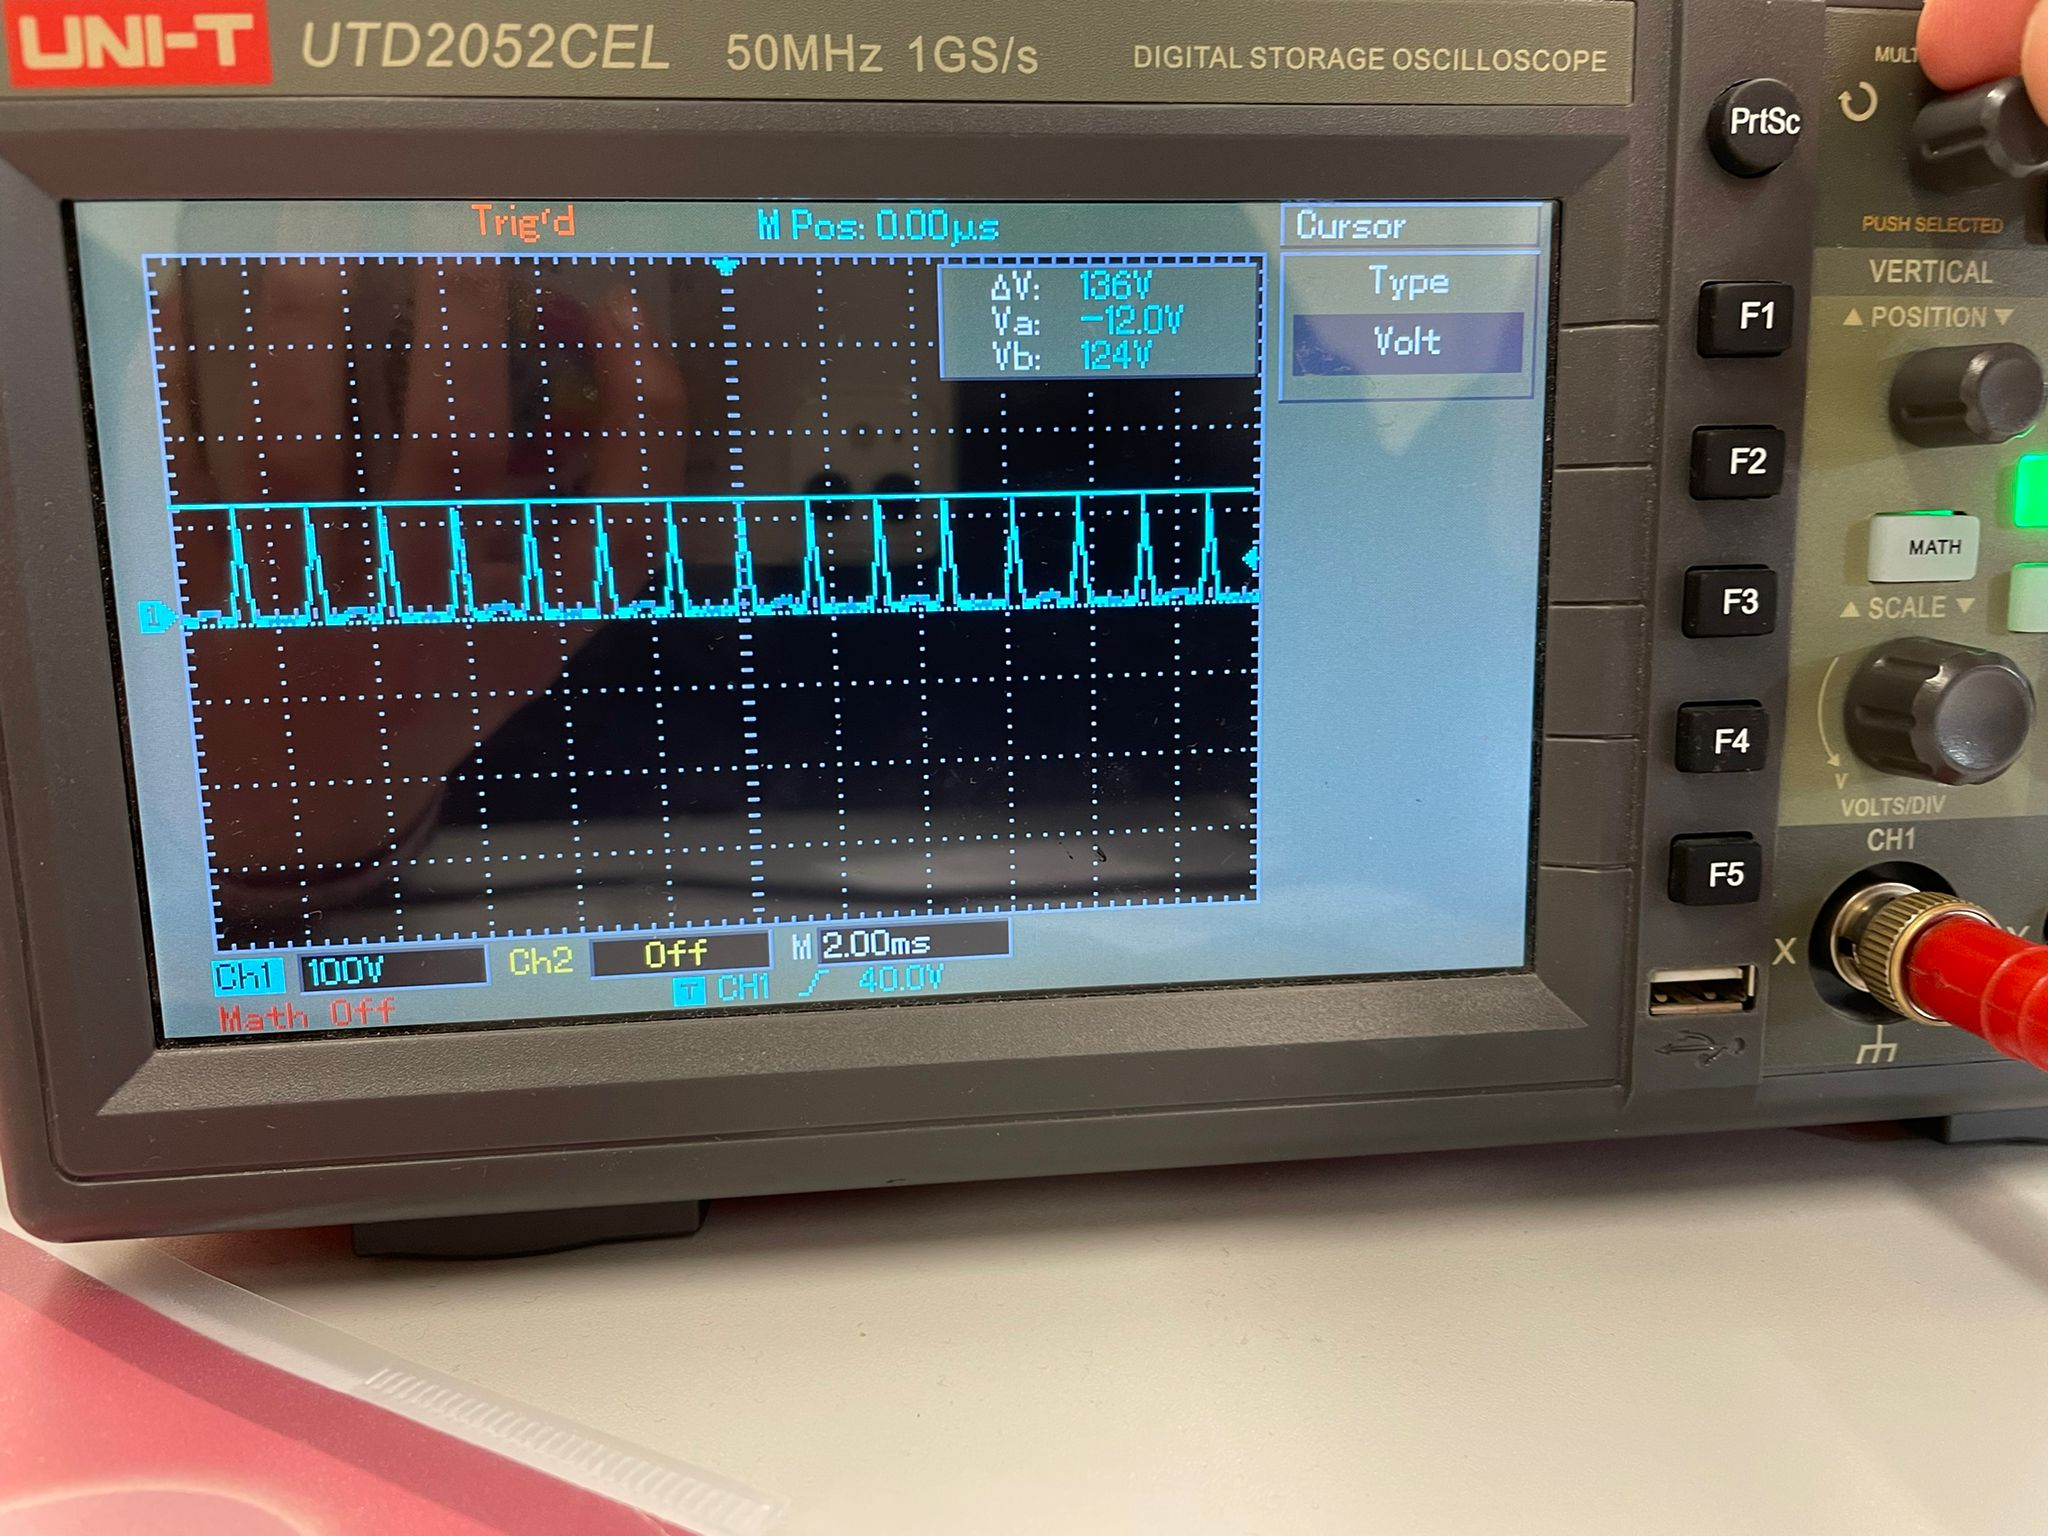
\includegraphics[scale=0.1]{content/norausch180.jpg}
    \caption{180° nicht verrauscht}
    \label{subfig:norausch180}
  \end{subfigure}
  \hfill
  \begin{subfigure}{0.48\textwidth}
    \centering
    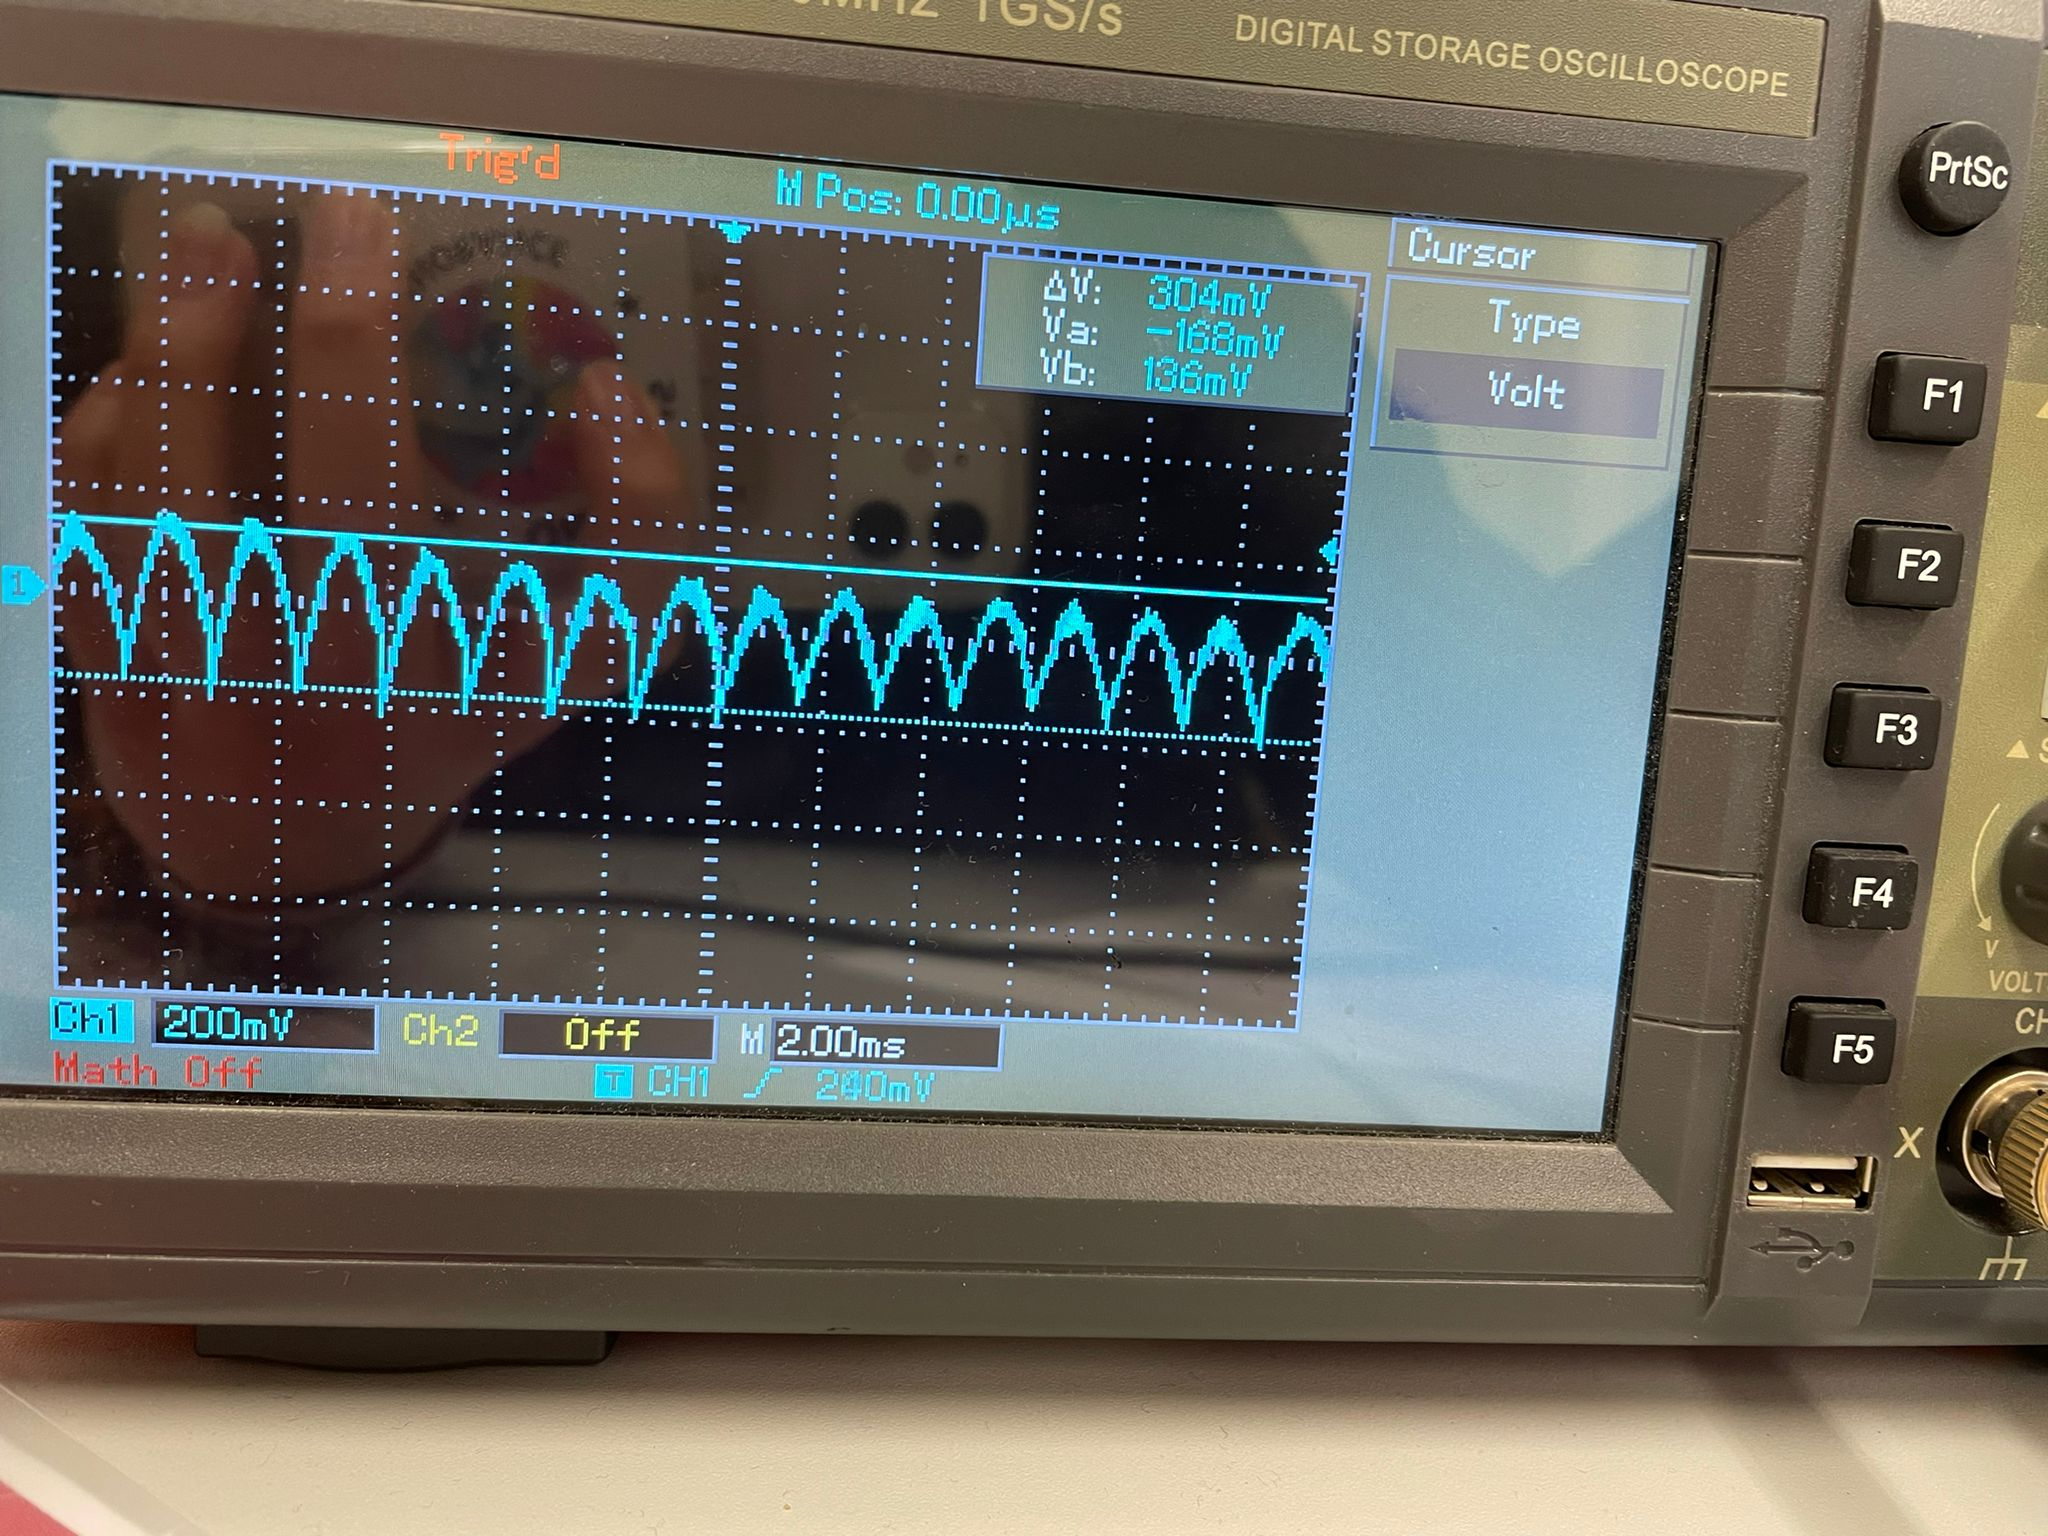
\includegraphics[scale=0.1]{content/rausch180.jpg}
    \caption{180° verrauscht}
    \label{subfig:rausch180}
  \end{subfigure}
\end{figure}
Die Daten der Messung am Lock-In-Verstärker aus \autoref{tab:DatenUnverrauscht} wurden in \autoref{fig:unverrauscht} und die Daten aus \autoref{tab:DatenVerrauscht} in \autoref{fig:verrauscht} aufgetragen
und eine Ausgleichsrechnungen nach
\begin{equation*}
  U = a\cos\left(b\varphi + c\right) + d
\end{equation*}
durchgeführt und ebenfalls im entsprechenden Diagramm aufgetragen.
\begin{table}
  \centering
  \caption{Die gemessenen Spannungen zur zugehörigen Phasenverschiebung des nicht verrauschten Signals.}
  \begin{tabular}{cc}
    \toprule
    {$\varphi \mathbin{/} °$} &
    {$U \mathbin{/} \unit{\volt}$} \\
    \midrule
      0 & 132\\
      30 & 216\\
      60 & 220\\
      90 & 216\\
      120 & 216\\
      150 & 188\\
      180 & 136\\
      210 & 216\\
      240 & 220\\
      270 & 212\\
      300 & 216\\
      330 & 192\\
      360 & 136\\
    \bottomrule
  \end{tabular}
  \label{tab:DatenUnverrauscht}
\end{table}
\begin{table}[H]
  \centering
  \caption{Die gemessenen Spannungen zur zugehörigen Phasenverschiebung des verrauschten Signals.}
  \begin{tabular}{cc}
    \toprule
    {$\varphi \mathbin{/} °$} &
    {$U \mathbin{/} \unit{\milli\volt}$} \\
    \midrule
      0 & 280\\
      30 & 256\\
      60 & 464\\
      90 & 512\\
      120 & 448\\
      150 & 336\\
      180 & 304\\
      210 & 368\\
      240 & 472\\
      270 & 480\\
      300 & 448\\
      330 & 384\\
      360 & 328\\
    \bottomrule
  \end{tabular}
  \label{tab:DatenVerrauscht}
\end{table}
\begin{figure}[H]
  \centering
  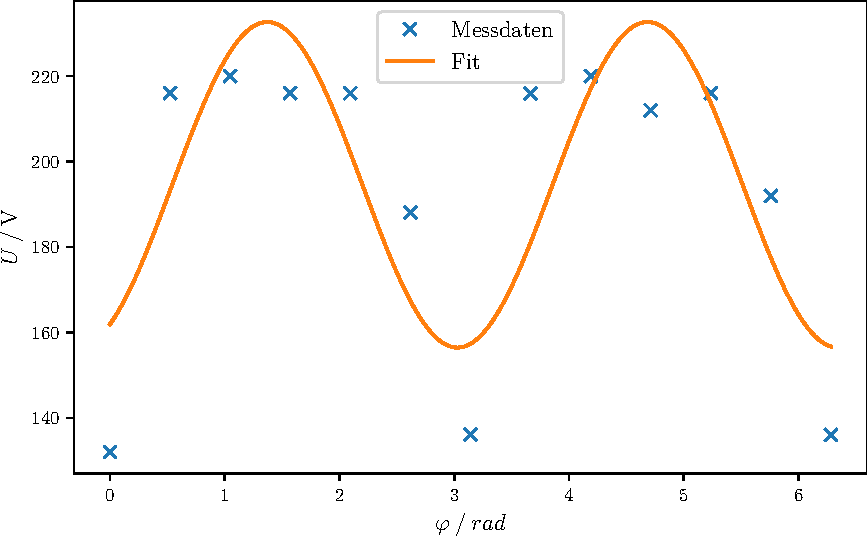
\includegraphics{unverrauscht.pdf}
  \caption{Die Messwerte aus \autoref{tab:DatenUnverrauscht} und die Ausgleichsrechnungen.}
  \label{fig:unverrauscht}
\end{figure}
\begin{figure}[H]
  \centering
  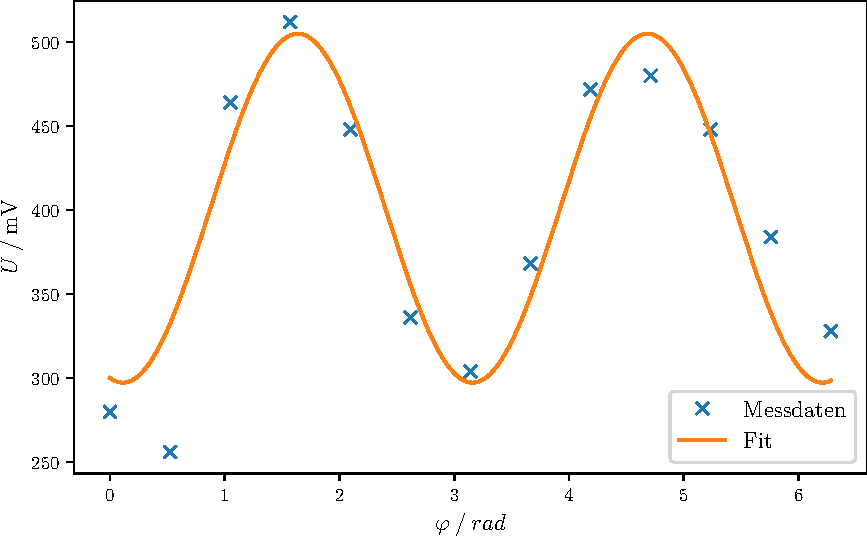
\includegraphics{verrauscht.pdf}
  \caption{Die Messwerte aus \autoref{tab:DatenVerrauscht} und die Ausgleichsrechnungen.}
  \label{fig:verrauscht}
\end{figure}
Die Parameter ergeben sich bei dem nicht verrauschten Signal zu
\begin{align*}
  a &= (-38,1099\pm 9,2292)\unit{\volt}\\
  b &= 1,8956\pm 0,1445\\
  c &= 13,1098\pm 0,5019\\
  d &= (194,5466\pm 7,1296)\unit{\volt}\\
\end{align*}
und für das verrauschte Signal ergibt sich
\begin{align*}
  a &= (103,8658\pm 13,7873)\unit{\milli\volt}\\
  b &= 2,0611\pm 0,0848\\
  c &= 2,9105\pm 0,3025\\
  d &= (401,1505\pm 10,5892)\unit{\milli\volt}.\\
\end{align*}
Die Amplidute der Spannung $U_0$ ergibt sich mit $U_0 = \frac{\pi}{2}a$ nach \autoref{eqn:U0} beim nicht verrauschten Signal zu
\begin{equation*}
  U_0 = (59,8629\pm14,4972)\unit{\volt}
\end{equation*}
und beim verrauschten Signal folgt
\begin{equation*}
  U_0 = (163,1520\pm21,6570)\unit{\milli\volt}.
\end{equation*}
\subsection{Photodetektorschaltung}
\label{subsec:PhotDet}
Es wurde die Schaltung wie in \autoref{fig:Prinzip_led} aufgebaut und die Messergebnisse aus \autoref{tab:DatenPhotoDet} in das in \autoref{fig:PhotoDet} zusehende Diagramm eingetragen.
Außerdem sind die Daten an die Funktionen
\begin{align*}
    U &= \frac{a_1}{r} + b_1\\
    U &= \frac{a_2}{r^2} + b_2\\
\end{align*}
\\
gefittet worden, um die Abhängigkeit der Lichtintensität vom Abstand zu erhalten. Bei diesen Ausgleichsrechnungen ergeben sich die Parameter zu
\begin{align*}
  a_1 &= 14,8304\pm 1,1554\\
  b_1 &= -53,1389\pm 10,1302\\
  a_2 &= 0,9299\pm 0,0264\\
  b_2 &= -9,1041\pm 2,6981\\
\end{align*}
Daraus und aus \autoref{fig:PhotoDet} folgt, dass sich die Funktion der Lichtintensität $\varpropto \frac{1}{r^2}$ verhält. Zudem wird \autoref{fig:PhotoDet}
entnommen, dass $r_{max}$ ca. zwischen $\SI{50}{\centi\meter}$ und $\SI{60}{\centi\meter}$ liegt, da die Kurve von dort an nicht mehr signifikant abfällt und nur noch
das Umgebungslicht gemessen wird, wordurch diese niemals gegen Null geht, sondern gegen einen konstanten Wert $>0$.
\begin{table}
  \centering
  \caption{Die gemessenen Spannungen zum zugehörigen Abstand der LED zum Photodetektor.}
  \begin{tabular}{cc}
    \toprule
    {$U \mathbin{/} \unit{\volt}$} &
    {$r \mathbin{/} \unit{\centi\meter}$} \\
    \midrule
      210.0 & 6.6 \\
      194.0 & 7.0 \\
      170.0 & 7.5 \\
      138.0 & 8.0 \\
      110.0 & 8.5 \\
      93.6 & 9.0 \\
      83.2 & 9.5 \\
      74.4 & 10.0 \\
      60.0 & 11.0 \\
      48.0 & 12.0 \\
      40.0 & 13.0 \\
      32.4 & 14.0 \\
      28.0 & 15.0 \\
      20.4 & 17.0 \\
      16.2 & 19.0 \\
      12.8 & 21.0 \\
      11.4 & 23.0 \\
      9.0 & 25.0 \\
      6.9 & 30.0 \\
      5.5 & 40.0 \\
      4.5 & 50.0 \\
      3.9 & 60.0 \\
    \bottomrule
  \end{tabular}
  \label{tab:DatenPhotoDet}
\end{table}
\begin{figure}
  \centering
  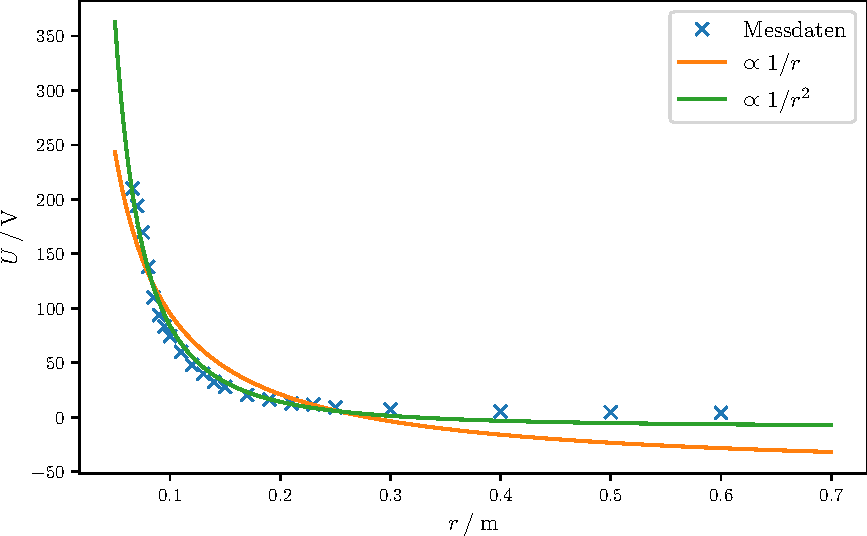
\includegraphics{Led-Messung.pdf}
  \caption{Die Messwerte aus \autoref{tab:DatenPhotoDet} und die Ausgleichsrechnungen in einem Diagramm aufgetragen.}
  \label{fig:PhotoDet}
\end{figure}
